\documentclass[11pt,a4paper]{book}
\usepackage[inner=2.5cm,outer=2.5cm,top=3cm,bottom=3cm]{geometry}
\usepackage{setspace}
\usepackage[hidelinks]{hyperref}
\usepackage[round]{natbib}
\usepackage{amsmath}
\usepackage{fontspec}
\usepackage{titlesec}
\usepackage{fancyhdr}
\usepackage{pdfpages}
\usepackage{microtype}
\setmainfont{Crimson Text}
\setsansfont{Open Sans}
\titleformat{\chapter}[display]{\Large\sffamily}{\chaptertitlename\ \thechapter}{0.5cm}{\normalfont\LARGE\bfseries\sffamily}[\vspace{0.5cm}\titlerule]
\titleformat*{\section}{\Large\bfseries\sffamily}
\titleformat*{\subsection}{\large\bfseries\sffamily}
\titleformat*{\subsubsection}{\bfseries\sffamily}
\setcounter{secnumdepth}{5}
\pagestyle{fancy}
\renewcommand{\sectionmark}[1]{\markright{\thesection\quad #1}}
\renewcommand{\chaptermark}[1]{\markboth{\chaptername\ \thechapter}{}}
\fancyhf{}
\fancyhead[LE,RO]{\sffamily\thepage}
\fancyhead[RE]{\sffamily\leftmark}
\fancyhead[LO]{\sffamily\rightmark}
\fancypagestyle{plain}{%
\fancyhf{}%
\fancyfoot[R]{\sffamily\thepage}%
\renewcommand{\headrulewidth}{0pt}
}
\bibliographystyle{copernicus}
%\setstretch{1.1}
\DeclareRobustCommand*\unit[1]
 {\ensuremath{%
   {\thinmuskip3mu\relax
    \def\mu{\text{\textmu}}\def~{\,}%
    \ifx\f@series\testbx\mathbf{#1}\else\mathrm{#1}\fi}}}
\begin{document}
\thispagestyle{empty}
\setstretch{1.2}
\begin{center}
\null
\vfill
\huge
\sffamily
\textbf{Comparing remotely sensed observations of clouds and
aerosols in the Southern Ocean with climate model
simulations}
\normalfont
\vfill
\Large
A thesis submitted in partial fulfilment of the requirements\\
for the Degree of Doctor of Philosophy
in the University of Canterbury\\
by Peter Kuma
\vfill
School of Physical and Chemical Sciences\\
University of Canterbury\\
Christchurch, New Zealand
\vfill
April 2020
\vfill
\end{center}
\clearpage
\thispagestyle{empty}
\normalfont
\null
\vfill
\noindent
\begin{center}
\large
Please consider the environment before printing this thesis.
\end{center}
\vfill
\noindent
Copyright \copyright\ 2016--2020 Peter Kuma and co-authors. This work is licensed under a Creative Commons Attribution 4.0 International License (\url{https://creativecommons.org/licenses/by/4.0/}).
\setstretch{1.0}

\clearpage
\fontsize{12pt}{16pt}\selectfont
\chapter*{Abstract}
\addcontentsline{toc}{section}{Abstract}

\noindent
Southern Ocean (SO) shortwave (SW) radiation biases are a common
problem in contemporary general circulation models (GCMs), with most
models exhibiting a tendency to absorb too much incoming SW radiation.
These biases have been attributed to deficiencies in the representation of
clouds during the austral summer months, either due to cloud cover or cloud
albedo being too low. They affect simulation of New Zealand (NZ) and global
climate in GCMs due to excessive heating of the sea surface and the effect on
large-scale circulation. Therefore, improvement of GCMs is necessary for
accurate prediction of future NZ and global climate. Currently the New
Zealand Earth System Model (NZESM), based on the UK Hadley Centre
Coupled Model version 3 (HadGEM3), is developed at the National Institute
of Water and Atmospheric Research (NIWA) and the University of
Canterbury. We performed ship-based lidar, radar, radiosonde and weather
observations on two SO voyages and processed data from multiple past SO
voyages. We used the observations and satellite measurements for
evaluation of NZESM and contrasting with the MERRA-2 reanalysis to better
understand the source of the problem. Due to the nature of lidar
observations (the laser signal is quickly attenuated by clouds) they cannot be
used for 1:1 comparison with a model without using a lidar simulator, which
performs atmospheric radiative transfer calculations of the laser signal. We
modify an existing satellite lidar simulator present in the CFMIP
Observational Simulator Package (COSP) for use with the ground-based lidars
used in our observations by modifying the geometry of the radiative transfer
calculations, Mie and Rayleigh scattering of the laser signal. We document
and make the modified lidar simulator available to the scientific community
as part of a newly-developed lidar processing tool Automatic Lidar and
Ceilometer Framework (ALCF), which enables unbiased comparison between
lidar observations and models by performing calibration of lidar backscatter,
noise removal and consistent cloud detection. We apply the lidar simulator
on NZESM model fields. Significant SW radiation errors in the SO of up to 21
Wm$^{-2}$ are shown to be present in the model. Using the lidar observations,
we find that the model underestimates overall cloud cover by about 9\% and
strongly underestimates boundary layer low-level stratocumulus cloud below
1 km and fog. The observed cloud was strongly linked to the boundary layer
stability and sea surface surface, while this relationship is weaker in the
model. We identify that these errors are not due to misrepresentation of
large-scale circulation, which is prescribed in our model based on global
satellite observations by nudging. We conclude that the problem is likely in
the subgrid-scale parametrisation schemes of the boundary layer, convection
and large-scale could. In order to address the deficiencies identified we
perform experimental simulations of NZESM with modifications of the
parametrisation schemes. By comparing high-resolution output produced by
the lidar simulator with the lidar observations and model atmospheric
profiles with radiosonde observations, we study boundary layer processes
which lead to underestimation of stratocumulus cloud and fog in the model,
with the aim of fixing the schemes based on physically-motivated reasons
without negatively affecting global cloud simulation in the model.

\clearpage
\includepdf[pages=-]{coauthorship_form_signed.pdf}
\clearpage
\chapter*{Acknowledgments}
\addcontentsline{toc}{section}{Acknowledgments}

I would like to thank
Adrian McDonald and Olaf Morgenstern for supervising my PhD;
University of Canterbury for providing me with the UC Doctoral Scholarship;
the New Zealand Deep South National Science Challenge for providing me with a
part of my scholarship and providing funding for our research;
NIWA and NeSI for providing access to their supercomputing resources and the Unified Model;
NIWA for making it possible to conduct Southern Ocean observations on R/V Tangaroa;
everyone who co-authored the papers which form Chapter 2 and Chapter 3:
Adrian McDonald, Olaf Morgenstern, Simon Alexander, John Cassano,
Sally Garrett, Jamie Halla, Sean Hartery, Mike Harvey, Simon Parsons, Graeme Plank,
Vidya Varma, Jonny Williams, Richard Querel, Israel Silber and Connor Flynn,
and everyone acknowledged in the Chapters;
my colleagues Alex Schuddeboom, Ethan Dale, Simon Parsons, Sean Hartery, Laura Revell and Graeme Plank for their insights, but also entertaining discussions;
all people of New Zealand, who have funded this research of the Earth's climate
in the remote region of the Southern Ocean for the benefit of the current and
future generations globally.


\tableofcontents
\listoffigures 
\listoftables
\chapter{Introduction}

Clouds represent one of the largest sources of uncertainty in estimating global
climate sensitivity \citep{williams2017}. Clouds over the ocean
are especially important for determining the radiation budget, due to the
low albedo of the sea surface compared to land.
Over the Southern Ocean (SO),
cloud cover exceeds 80\%, with predominantly boundary layer clouds \citep{mace2009}.
Due to its large influence on circulation and atmospheric transports in the
Southern Hemisphere, the SO is important for global climate. Unlike
most other places on the globe, it is largely unaffected by sources of
continental and anthropogenic aerosols, is dominated by a strong circumpolar
vortex, and its southern boundary is a permanently ice-covered continent,
which could mean that global parametrisations do not apply very well in this
region.
SO south of 30$^\circ$S accounts for about 43\% of anthropogenic CO$_2$ and 75%
of excess heat uptake \citep{frolicher2015}.
Observations in the SO are sparse, which limits the accuracy
of simulations by numerical weather prediction (NWP) models and general
circulation models (GCMs).
Globally, clouds have a predominantly cooling effect on the climate due to reflection
of sunlight, which exceeds the warming effect due to absorption of thermal
radiation from the surface, estimates identify 18 Wm$^{-2}$ of cooling relative to a cloud-free atmosphere
\citep{zelinka2017}. This effect is about 5 times as large as heating from
a doubling of CO$_2$, which highlights the importance of cloud cover in modulating
global climate. Nearly all climate models predict cloud feedback to be positive,
i.e. amplification of warming with increasing CO$_2$ concentration.

\begin{figure}[t]
\centering
\includegraphics[width=\textwidth]{fig/trenberth-fassulo-sw-bias.png}
\caption[Biases in the TOA net radiation down]{
Biases in the TOA net radiation down relative to observations regionally for
1990--99
in $Wm^{-2}$, where stippled (hatched) regions correspond to regions
in which at least three quarters of the models share a common
positive (negative) bias. (right) The model zonal mean is given
(dots) with the 25th to 75th percentile range (lines) over land (red),
ocean (blue), and all (black) surfaces. \textbf{Adopted from
\cite{trenberth2010}.}
}
\label{fig:trenberth-fassulo-sw-bias}
\end{figure}

Shortwave (SW) radiation bias over the SO of up to 30 Wm$^{-2}$ is a
well-documented problem in current NWP models and GCMs
\citep{trenberth2010} (Fig. \ref{fig:trenberth-fassulo-sw-bias}),
and it has been the subject of many studies.
It manifests both as a bias in SW radiation reaching the surface and as a
SW reflectivity bias at the top of atmosphere (TOA).
\cite{bodas-salcedo2014} evaluated SW bias in a number
of GCMs and found a strong SW bias is a very common problem, leading to
overestimated sea surface temperature (SST) in the SO.
\cite{trenberth2010} noted that a poor representation of clouds might lead to
unrealistic projections for the Southern Hemisphere. This bias is linked to
large-scale model errors such as a double-intertropical
convergence zone \citep{hwang2013}, position of the midlatitude jet and
meridional energy transport \citep{mason2014}.
The reasons for the observed SW radiation bias
can be numerous, concurrent and compensating.
As noted by \cite{kelleher2019}, cloud biases in the SO can arise either
as a result of biases in large-scale dynamics, or cloud parametrisation.
To summarise, they can range
from microphysical to large-scale dynamics and be due to misrepresentation of:
cloud fraction, cloud optical depth, frequency of cloud regimes or types,
cloud vertical distribution and overlap, cloud horizontal distribution
and homogeneity, cloud phase and supercooled liquid content, surface albedo
(sea ice vs. water), moisture fluxes, large-scale circulation, extratropical
and polar cyclones, weather regimes, direct and indirect aerosol effects,
radiative transfer parametrisation, boundary layer turbulence and convection,
among others.

The New Zealand Earth System Model (NZESM)
is a relatively new earth system model based on the UK climate model HadGEM/UK Earth System Model (UKESM)
\citep{williams2016}, whose aim is to improve climate predictions for
Aotearoa/New Zealand. Reducing SO model biases is essential for
achieving this aim. \cite{walters2017}
showed that a clear and extensive SW radiation bias over the SO
is present in the atmospheric component of the model Global Atmosphere version 6.0 (GA6.0) compared to satellite
radiation budget observations by the Clouds and the Earth's Radiant Energy
System (CERES) \citep{wielicki1996}. The bias in the context of the UK Met Office
models has been studied by \cite{bodas-salcedo2012} by assessing cloud
regimes in cyclones.
Using observations by the International Satellite Cloud Climatology Project
(ISCCP) \citep{rossow1999},
Multi-angle Imaging SpectroRadiometer (MISR) \citep{diner1998}, Moderate Resolution Imaging Spectroradiometer (MODIS) \citep{salomonson2002},
Cloud-Aerosol Lidar and Infrared Pathfinder Satellite Observation
(CALIPSO) \citep{winker2010} and CloudSat \citep{stephens2002} satellites,
they found that the model underestimates optical depth of stratocumulus and
mid-topped clouds. Recently, \cite{davies2017} studied boundary layer
clouds in the SO compared to the Northern Hemisphere,
with a focus on supercooled liquid in clouds and cloud homogeneity.
They noted that boundary layer clouds are a likely explanation for the bias
due to their large fractional coverage over the SO.
Examination of cloud cover in the NZESM against passive satellite instruments
was performed by \cite{schuddeboom2017,schuddeboom2019} and is an ongoing effort.

While some authors focused on cloud distribution, others
emphasised the role of microphysics, especially supercooled liquid content.
Because supercooled liquid has a higher SW reflectivity than the equivalent amount
of ice particles (in terms of mixing ratio), it has a positive effect on cloud albedo.
\cite{morrison2011} studied the occurrence of supercooled liquid in clouds
over the SO using observations by MODIS and
found that it is present year-round in low clouds at temperature as low as
--40 $^{\circ}$C.
\cite{lawson2014} noted that supercooled liquid is often
underestimated in the Antarctic in GCMs, and mixed clouds can occur at
--32 $^{\circ}$C.
They showed that increasing supercooled liquid in the
Community Earth System Model (CESM) leads to a cloud radiative effect (CRE)
increase of 7.4 Wm$^{-2}$ over Antarctica. More recently, \cite{kay2016}
managed to fix the SW radiation bias in the CESM by increasing supercooled liquid
in shallow convective clouds, and notably they also needed to reduce a
compensating tropical SW radiation bias to maintain global radiation balance
in the model.
\cite{bodas-salcedo2016} found supercooled liquid to be abundant in
the SO in summer and contribute about 30\% to the reflected
SW radiation.
\cite{noh2019} developed an algorithm for detecting mixed-phase cloud with
liquid top in the SO using Himawari geosynchronous (GEO) satellite data, which are thought
to be common in the region, but difficult to detect with passive satellite
instruments. They focused on liquid‐top mixed‐phase clouds. In their case studies, they found both supercooled liquid
and mixed clouds with liquid top over the SO south of Australia and
New Zealand and noted that their algorithm may complement active instruments
in detecting mixed cloud.

Several field campaigns were performed in the SO in recent years:
Clouds, Aerosols, Precipitation, Radiation, and Atmospheric Composition over the Southern Ocean (CAPRICORN) \citep{mace2018a,mace2018b}, Measurements of Aerosols, Radiation and Clouds over the Southern Ocean (MARCUS) \citep{mcfarquhar2016},
the Southern Ocean Clouds, Radiation, Aerosol Transport Experimental Study (SOCRATES) \citep{mcfarquhar2014} and the Macquarie Island Cloud and Radiation Experiment (MICRE) \citep{demott2018}.
The SOCRATES campaign consisted of 15 flights of GV HIAPER and a voyage
of R/V Investigator from Hobart, Tasmania in January--February 2018,
organised by the National Science Foundation (NSF) and the
National Center for Atmospheric Research (NCAR). \cite{gettelman2020}
analysed cloud microphysical observations from these flights compared
to nudged CAM6 simulations, and found that CAM6 represents cloud properties
relatively well, and observed supercooled liquid clouds extensively in cold
sectors of cyclones. They found the representation of supercooled liquid
better than in CAM5 due to a scheme dependence on the available ice nuclei.
They found 50\% differences in ice water path (IWP) and liquid water path (LWP)
between CAM5 and CAM6. Their model simulates cloud droplet size distribution
prognostically and they found a satisfactory agreement with the in situ
airborne observations.
\cite{mace2018a} analysed cloud observations collected on the second CAPRICORN
voyage of R/V Investigator from Hobart, Tasmania to 53$^\circ$ S in March--April 2016.
In their radar and lidar observations, low cloud below 2 km was predominant
during the voyage and the total lidar cloud fraction was 76\%, compared to 87\%
in CloudSat--CALIPSO in the region and time of year in 2007--11, with
more high clouds identified by CloudSat--CALIPSO.
They also found that about 30\% of cloud is detected by a ship-based lidar but not
a radar due to low sensitivity of the radar. In terms of cloud phase,
they found that ice-phase processes occur 20-40\% more often than implied
by CALIPSO due to attenuation of the signal at the cloud top. Thus, one should
perhaps be cautious when using active satellite
products as a reference for supercooled liquid cloud evaluation in GCMs
in this region. They performed 1--2 daily soundings and found MERRA-2 about
1.2 K warmer and 8\% drier. They note that unlike the lidar, the radar is unable
to reliably detecect cloud base height due to frequent precipitation, which
cannot be distinguished from cloud.
\cite{mace2018b} studied stratocumulus clouds occurring during the CAPRICORN
voyage. They characterise them as tenuous, supercooled, rarely drizzling
and present in cold air advection. They quantify their water path at 15--25 \unit{gm^{-2}},
effective radius at 8 \unit{\mu m}, number concentration at 20 \unit{cm^{-2}} and optical
depth 3--4. It is probably notable, however, that these values can be different
in the high-latitude SO, not reached by the CAPRICORN voyage. They hypothesise
that these non-precipitating stratocumulus clouds are responsible for majority
of the SO shortwave radiation biases identified in GCMs.
The MARCUS field campaign was conducted between November 2017 and March 2018
on \textit{Aurora Australis}. It was focused on collecting biogenic INP concentrations in the region,
but a range of ARM instruments were deployed on this ship.
\cite{zheng2019} analysed warm air advection events on the voyages and found
that they induce highly-stratified cloud-topped marine boundary layer with
stratiform clouds.

Multiple observational datasets are available for assessing the SO biases,
largely consisting of satellite datasets, and a relatively few ship- and
land-based datasets due to the very large costs and operational difficulties
of field campaigns in this remote and extreme-weather region. 
Satellite observations provide the most complete record both spatially and
temporally, although they do not provide historical records prior to
1960s and past observations are limited by instrument capabilities and
the availability of derived products. They have been utilised by most studies
of clouds in the SO and globally. Satellite instruments are very diverse, though only a few
datasets are readily available for studying clouds.
Operational GEO satellites provide near-continuous temporal
coverage,
which makes them ideal for studying clouds, but they have a limited use in
high-latitude regions such as the SO. In combination with operational polar-orbiting
low Earth orbit (LEO) satellites such as the NASA
Polar Operational Environmental Satellites (POES),
they have been used to produce a very long-term (1983--present) cloud-oriented
dataset ISCCP
\citep{schiffer1983}. However, this dataset is limited by
a small number of spectral channels of the Advanced Very High Resolution Radiometer
(AVHRR). Other extensive
cloud datasets include MODIS
on board of the NASA Afternoon Train (A-Train) satellites Aqua and Terra
and the Extended AVHRR Polar Pathfinder (APP-x) \citep{meier1997}. Other notable instruments available
for studying clouds include MISR
and passive
microwave sensors, due to their ability to observe cloud liquid water,
total column water vapour, vertically-resolved temperature profile, and
ability to see through clouds, even though their relatively low spatial
resolution makes passive microwave instruments less popular than passive visible (VIS) and infrared (IR)
instruments.
Passive VIS and IR satellite observations of clouds are ideal due to their high
spatial and temporal resolution, but have a number problems globally and some
specifically in polar latitudes \citep{bromwich2012}:

\begin{itemize}
\item Passive instruments can only observe the highest layer of clouds, unless
the layer is semi-transparent, meaning that cloud vertical structure is
poorly measured with passive instruments.
\item It is difficult to discern clouds from surface ice and snow
in the VIS spectrum due to similar albedo and in the IR
spectrum due to similar
temperature and frequent inversions.
\item Poor detection of semi-transparent high clouds, falsely classified as
mid-level clouds \citep{haynes2011}.
\item Lack of sunlight limits polar wintertime SW measurements.
\end{itemize}

\begin{figure}[t]
\centering
\includegraphics[width=\textwidth]{fig/space_vs_surface_lidar.png}
\caption[Spaceborne vs. surface lidar scattering ratio]{
\textbf{(a), (a')} Spaceborne vs. \textbf{(b), (b')} surface lidar scattering ratio
(SR) simulated based on the New Zealand Earth System Model (NZESM) output in
year 2017 at a lidar wavelength of 532 nm.
\textbf{(a), (b)} show SR at a model level corresponding to approximately 300 m
above sea level (ASL) over the sea, and \textbf{(a'), (b')} show an SR histogram by height.
}
\label{fig:surface-vs-spaceborne-lidar}
\end{figure}

Active satellite instruments are affected by signal attenuation by
optically thick
clouds (lidar), ground clutter (radar), and compared to passive instruments they have smaller spatial coverage,
shorter historical record and a small number of spectral bands, limiting their
ability to determine cloud microphysical properties \citep{noh2017,mace2018a,mace2018b,gettelman2020}.
In addition to spaceborne observations, ground-based and in situ
observations can provide an important complementary view of clouds from below.
Figure \ref{fig:surface-vs-spaceborne-lidar} shows that scattering ratio (SR)
(the ratio of total backscatter to molecular backscatter)
in the boundary layer measured by a lidar is much higher when measured by 
a ground-based lidar than a spaceborne lidar due to obscuration by higher-level
cloud.
Ground-based and in situ instruments include radars, ceilometers, lidars,
pyranometers, sky cameras, radiosondes, dropsondes, in situ aerosol measurements
(cloud condensation nuclei and ice nuclei) and airborne observations from
drones, weather balloons, kites and aircraft. These observations are logistically
difficult and expensive, and are generally sparse in the SO, with
limited time periods and limited historical records. The use of ground-based and
in situ observations alone for assessment of GCMs is difficult due to their
small representativeness of climatic conditions, and therefore there
is a risk of tuning the model to the specific conditions occurring during a
case study \citep{jakob2003}. Deployments on ships of opportunity can make these types
of observations more cost-efficient and common.

Different processing of observations from the same instrument can lead
to different results, for example the
GCM-Oriented CALIPSO Cloud Product (GOCCP) relative to the standard
Cloudsat--CALIPSO products \citep{chepfer2010}.
Different thresholds can be applied which define what 'cloud' is,
and cloud detection is affected by targeting a particular false alarm ratio,
such as 5\% as in the CloudSat--CALIPSO dataset \citep{hagihara2010}.
Probability of detection (sensitivity) then depends on the receiver operating
characteristic (ROC) curve, which in turn depends on instrument
noise. Instrument noise and bias can vary over lifetime of the instrument,
or between instruments of multi-instrument datasets such as ISCCP.
A problem with different processing
algorithms was noted by \cite{martucci2010}, who compared
manufacturer-supplied cloud base height (CBH)
determination between co-located Vaisala CL31 and Jenoptik CHM 15k ceilometers
and found a poor agreement, and developed a new algorithm for determining
CBH which leads to consistent height between the two instruments.

Due to the reasons outlined above, a combination of multiple satellite passive, active,
ground-based and in situ observations are needed to comprehensively assess
cloud climatology and biases. This has been also noted by other authors:
\cite{williams2017} evaluated cloud representation in the UK Met Office
Unified Model (UM) using a multi-dataset and multi-diagnostic approach, and
highlighted the
importance of using multiple instruments due to compensating errors in GCMs.
While use of single or combined satellite observations to assess model
performance is common in many studies,
combination of ground-based and spaceborne instruments is less common.
For example, \cite{muhlbauer2015} studied cirrus clouds using A-Train
observations (CloudSat, CALIPSO, MODIS, CERES), ground-based
Atmospheric Radiation Measurement (ARM) radar and aircraft observations.
\cite{zhang2017} performed a comparison of satellite and ground-based cloud
observations at an ARM site.

Comparison between models and observations cannot always be performed directly,
especially if observations do not produce fields equivalent to model quantities.
In such cases observations can be mapped to model fields by inversion algorithms,
but this may be unreliable
due to a large number of factors involved and a limited view of the instrument
(parts of the atmosphere obscured by clouds).
Conversely, model fields can be mapped to observations by instrument simulators,
and this approach has been used extensively in a number of studies.
Satellite simulators such as the Cloud Feedback Model Intercomparison Project (CFMIP) Observation Simulator Package (COSP)
\citep{bodas-salcedo2011} solve the problem
by transforming model fields to observed fields, which can then
be compared directly or statistically.

We provide a further literature review in Chapter 2.

\section{Objectives}
\label{sec:objectives}

Our objectives are aligned with the New Zealand Deep South National
Science Challenge (DSC), whose mission is to \textit{`enable New Zealanders to adapt,
manage risk, and thrive in a changing climate'}, and is
broadly in line with the current international research in the area
such as the Southern Ocean Clouds
Radiation Aerosol Transport Experimental Study (SOCRATES) \citep{mcfarquhar2014}.
Here, we focus on complementing other studies evaluating
representation of clouds, aerosols and cloud-aerosol interaction in the SO,
but also taking into consideration the Southern Hemisphere and global processes,
with a particular focus on utilising in situ measurements
available from intensive observation periods (IOPs), complemented by land-based
stations. For this
purpose the COSP simulator needs to be extended to support these
instruments. A ground-based observations need to be
complemented by satellite observations, especially the global radiation budget
measurements by CERES.
Other diagnostic means include
case studies, by which we can ensure that any improvements are due to
the right physical reasons rather than just improving statistics by mutually
compensating model errors. Our particular focus is therefore on linking
observed biases to model processes. 
We shall try to evaluate specific deficiencies in the NZESM subgrid-scale
parametrisations affecting clouds and radiative transfer, in order to
determine the relative importance of cloud macrophysical and microphysical
characteristics in the observed biases. This has been explored to some extent
by other authors, but not always in the context of the UM or the NZESM,
where the causes can be different.
While our focus is on evaluation of the NZESM, contrasting with other
models, such as atmospheric reanalyses is useful.
We shall focus on biases in the SO and the
Antarctic, but pay attention to any processes relevant to the Southern
Hemisphere and globally.
Adjacent to our study will be development of a publicly-available dataset
of in situ observations in the SO based on previous and new SO voyages
and permanent stations collected by the University of Canterbury and our
collaborators.
Our main objectives are outlined below:

\begin{enumerate}
\item Participate on SO IOPs
with the aim of collecting atmospheric observations for model evaluation.
\item Collate and post-process the existing and new SO in situ datasets.
\item Extend the COSP lidar simulator with a ceilometer and ground-based lidar
simulator for instruments deployed on the SO voyages.
\item Use in situ and satellite observations in conjunction with the lidar simulator
to evaluate SO cloud biases in the NZESM.
\item Perform experimental simulations of the NZESM with the aim of
improving the simulation of SO clouds relative to the observations.
\end{enumerate}

\section{Methods}

Achieving our objectives will require a number of modelling and
observational resources. As outlined here and discussed in
a greater detail in Chapter 2, 3 and 4, these include access to the model output
and
code of the NZESM, the COSP simulator, publicly-available reanalyses,
 in situ SO observations and publicly-available
satellite datasets.

\subsection{New Zealand Earth System Model}

The NZESM is an actively developed branch of HadGEM/UKESM, with the
aim of improving the atmosphere, ocean and cryosphere simulation affecting
Aotearoa/New Zealand
\citep{williams2016}. Development is done by the National Institute of Water and
Atmospheric Research (NIWA) in Wellington and the University of Canterbury.
The NZESM is a fully coupled atmosphere-ocean model, including land surface
and sea ice. The parent model UKESM \citep{walters2017} is planned to participate
in the 6th Climate Model Intercomparison Project (CMIP6) \citep{eyring2016,meehl2014},
which shall eventually contribute to the upcoming
Intergovernmental Panel on Climate Change (IPCC) 6th
Assessment Report (AR6). Participation of the NZESM in the CMIP6 is currently not
envisioned, although any improvements achieved will be continuously contributed
to the parent model.

Apart from a standard free-running mode, it is possible to run the NZESM
in a nudged mode, continuously modulated by observed meteorological
conditions using the ERA-Interim reanalysis \citep{dee2011} and prescribed SST and sea ice
by the HadISST dataset \citep{rayner2003}.
A nudged run can be useful for comparison with instantaneous values of
observational data taken during the simulated period,
as opposed to long-term statistics. The model fields can be exported
at arbitrary intervals down to the model time step of 20 minutes.

\subsection{CFMIP Observation Simulator Package}

COSP \citep{bodas-salcedo2011} is a satellite instrument simulator package
for atmospheric model evaluation developed as part of
the CFMIP \citep{bony2011},
whose purpose is to generate pseudo-measurements and statistics from model fields, which can
then be compared to real
measurements. A direct comparison without a simulator is often not possible
due to a limited field of view (FOV) of the instrument and attenuation by atmospheric
constituents (clouds, aerosols, gases), which is a wavelength-dependent process.
COSP was utilised in evaluation of GCMs in the
Coupled Model Intercomparison Project Phase 5 (CMIP5) \citep{taylor2011}.
COSP contains multiple simulators of different instruments:
ISCCP, MODIS, MISR, CloudSat, CALIPSO, a MilliMeter-wavelength Cloud Radar
(MMCR)/Ka-Band ARM Zenith Radar (KAZR) ground-based radar
and the Radiative Transfer for Television Infrared Observation Satellite (TIROS)
Operational Vertical Sounder (TOSV) (RTTOV).
Notably, radar observations are simulated by the QuickBeam simulator
\citep{haynes2007} and lidar (CALIPSO) observations are simulated
by the Active Remote Sensing Simulator (ACTSIM) \citep{chepfer2008}. In general, these may need
to be tuned for any particular instrument being simulated due to different
wavelengths, signal modulation, view and error characteristics.
COSP allows for comparison of instrument quantities
(backscatter, radar reflectivity), or derived products
(cloud top/base, cloud phase, ...) between the model and observations.
An exact co-located comparison is limited by the relatively low spatial and
temporal resolution
of GCMs, and pseudo-observations need to be made on subcolumns generated by
a cloud generator. Algorithms for calculating derived products are generally not
available, and datasets such as CALIPSO-GOCCP were developed for the purpose
of comparison of equivalent quantities from observations and the simulator
\citep{chepfer2010}.
COSP can be run either online (inside the model) or offline,
when fields from a model are provided to COSP after completing the simulation.
Running the simulator offline allows for rapid modification
and testing of code. Cloud overlap in COSP is treated by the Subgrid Cloud Overlap Profile Sampler
(SCOPS) \citep{webb2001}, which generates subcolumns based on the grid cell
cloud fraction and precipitation fluxes. Either random or maximum-random cloud overlap
\citep{geleyn1979,ritter1992} is assumed,
whereby cloud in the adjacent layers overlaps maximally, and cloud separated
by clear layers overlaps randomly.

ACTSIM is a lidar simulator integrated in COSP
\citep{chepfer2008,chiriaco2006}. In the current implementation it simulates a
spaceborne lidar with a wavelength of 532 nm, aimed at simulating the CALIOP
instrument on CALIPSO. The simulator produces attenuated volume backscatter
coefficient, which can be compared directly with measurements from a lidar.
Support for a ground-based ceilometer such as Lufft CHM 15k or Vaisala CL51
will require modification of ACTSIM. Firstly, the viewpoint from
the ground means that the lidar signal passes through atmospheric layers in a reversed
order relative to what is assumed for a spaceborne lidar. Secondly,
wavelength of our instruments is different from CALIOP (1064 nm and 910 nm),
which requires re-calculation of the Mie and Rayleigh scattering coefficients.

\subsection{In situ observations in the Southern Ocean}

\begin{figure}[t]
\centering
\includegraphics[width=\textwidth]{fig/instruments.jpg}
\caption{
Instruments deployed on Southern Ocean voyages and stations.
}
\label{fig:instruments}
\end{figure}

In situ SO observations are essential for improving the model SO biases.
A set of SO datasets have been collected by the University of Canterbury
and partner organisations by deploying our instruments on a number
of voyages of opportunity as well as conducting IOPs:

\begin{itemize}
\item \textit{Aurora Australis} voyages to Casey, Davis and Mawson, Antarctica (2015--2016).
\item Macquarie Island station (2016--2018).
\item HMNZS \textit{Wellington} voyages to the Ross Sea (2016).
\item RV \textit{Nathaniel B. Palmer} voyage NBP1704 to the Ross Sea (2017).
\item RV \textit{Tangaroa} voyages TAN1502, TAN1503 (2015), TAN1702 (2017) and TAN1802 (2018)
to the Ross Sea, Chatham Islands, the Campbell Plateau and the Ross Sea, respectively.
\end{itemize}

\noindent
The author participated on field measurements on the TAN7102 and TAN1802 voyages and the deployments
on the HMNZS \textit{Wellington} and the NBP1704.
In addition to the datasets outlined above we have access to a set of
ceilometer and lidar observations from the following land-based locations in
Aotearoa/New Zealand:

\begin{figure}[t]
\includegraphics[width=\textwidth]{fig/chm15k_profile.png}
\caption[Lufft CHM 15k ceilometer volume backscattering coefficient profile plot]{
A Lufft CHM 15k ceilometer volume backscattering coefficient profile plot
and corresponding sky camera images collected on the TAN1702 voyage
on 23 March 2017.
}
\label{fig:chm15k-profile}
\end{figure}

\begin{itemize}
\item \textbf{Cass}, a deployment of a Vaisala CL51 ceilometer at a station in the
Southern Alps, Aotearoa/New Zealand.
\item \textbf{Lauder}, a dataset of a Sigma Space MiniMPL lidar and a Vaisala CL31
ceilometer observations at a station in Aotearoa/New Zealand made available by NIWA.
\item \textbf{Christchurch}, a deployment of a Lufft CHM 15k and a Sigma Space MiniMPL on the
Ernest Rutherford building of the University of Canterbury, Aotearoa/New
Zealand.
\end{itemize}

Observations collected on the voyages include remote sensing with ceilometers and lidars,
a micro rain radar, radiosonde profiles, automatic weather station (AWS) data (temperature, relative humidity,
wind, SST, radiometer...), UAV and tethered balloon soundings and
aerosol concentration (Fig. \ref{fig:instruments}.
Below, we briefly describe the instruments.

\textit{Lufft CHM 15k} is an IR ceilometer operating at a single wavelength of
1064 nm, which makes it suitable for observation of cloud droplets and
ice particles of similar size and boundary layer aerosol.
The primary purpose of a ceilometer
is observation of CBH, although other atmospheric features
such as boundary layer height, visibility, precipitation and multiple
cloud layers can be detected as well using a suitable algorithm. The
primary measured quantity is attenuated volume backscattering coefficient
$\beta$ (km$^{-1}$sr$^{-1}$), which
can also be used for a direct comparison with a ceilometer simulator.
The instrument allows for an easy deployment
in adverse conditions, such as on ships.
The ceilometer records data in the NetCDF format \citep{rew2006},
which makes it easy
for processing by various data analysis tools.
The averaging period of the instrument is 2 s. This provides spatiotemporal
resolution much greater than a GCM. Averaging over longer time periods can be applied to improve the signal-to-noise ratio (SNR).

\textit{Vaisala CL51} is an IR ceilometer operating a
wavelength of 910 nm. Similar to Lufft CHM 15k, it is suitable for observation
of cloud droplets and ice particles. The averaging period is 6 s.
The firmware contains onboard detection of multiple cloud layers and
visibility by a standard algorithm and a Sky Condition Algorithm (SCA).
Two-dimensional backscatter profiles are recorded in ASCII-encoded data files.

\textit{Metek MRR-2} is a micro rain radar, operating at a microwave frequency of
24.230 GHz, i.e. wavelength of 12.38 mm. The wavelength makes it suitable
for observation of liquid and ice precipitation. This instrument can
be used alongside the Vaisala CL51 instrument to detect period of time with
precipitation and rain rate. A Metek MRR-2 was deployed on the TAN1702, TAN1802
and HMNZS \textit{Wellington} voyages.

A sky camera was used as an ancillary instrument providing a visual
perspective of the atmospheric conditions (type of cloud, fog,
precipitation), as well as a primary instrument for determining cloud fraction.
Our deployments included
an off-the-shelf time lapse camera Brinno BCC200 (as a low-cost but
satisfactory solution) and a fisheye-lens camera.
The sampling period can be chosen from a wide range of values; we have
determined that a 5-minute interval is sufficient.
Figure \ref{fig:chm15k-profile} shows an example backscatter profile plot
from the TAN1702 voyage, combined with sky camera images. 
In addition to CBH, these measurements provide a wealth
of information about the cloud type, the vertical extent, optical thickness,
precipitation, fog and boundary layer aerosol. Some of these, as well
as satellite cloud observations in the Ross Sea region, were analysed
by co-authored studies: \cite{klekociuk2018,jolly2018,hartery2020a,hartery2020b}.

Preliminary analysis of multiple voyage datasets indicates that low cloud
below 2 km constitutes the majority of cloud in the summertime in the SO
(Fig. \ref{fig:cbh}). Preliminary results from the TAN1802 voyage also
show a very high cloud fraction of 94\% and a strong peak of boundary layer
cloud below 1 km above sea level (ASL) (Fig. \ref{fig:tan1802-stats}a), the predominance
of stratus (52\%) and stratocumulus (30\%) clouds (Fig. \ref{fig:tan1802-stats}b), predominantly
near-zero SST (Fig. \ref{fig:tan1802-stats}c) and near-surface air temperature below SST
(Fig. \ref{fig:tan1802-stats}d, e). These results suggest a cold boundary layer
destabilised by relatively warm SST and subsequent formation of
low stratus and stratocumulus cloud.

\begin{figure}[t]
\includegraphics[width=\textwidth]{fig/cbh.pdf}
\caption[Cloud base height distribution]{
Cloud base height distribution on the HMNZS \textit{Wellington} 2016, TAN702 and NBP1704
voyages derived with a Lufft CHM 15k ceilometer observations (as determined by
the instrument's firmware).
}
\label{fig:cbh}
\end{figure}

\begin{figure}[t]
\includegraphics[width=\textwidth]{fig/tan1802_stats.pdf}
\caption[Statistics calculated from observations collected on the TAN1802 voyage]{
Statistics calculated from observations collected on the TAN1802 voyage.
\textbf{(a)} cloud occurrence as a function of height, the 68-th and
90-th percentiles and the total cloud fraction (CF) calculated from a Lufft CHM 15k ceilometer observations.
\textbf{(b)} cloud type and cloud cover (octas) occurrence
in \% calculated from human observations. Histograms of \textbf{(c)} sea surface temperature (SST), \textbf{(d)} air temperature
and \textbf{(e)} SST - air temperature calculated from the automatic
weather station (AWS) data.
}
\label{fig:tan1802-stats}
\end{figure}

\subsection{Satellite radiation budget observations}

Earth radiation budget (ERB) observations are central for assessment and development
of GCMs. LEO satellite observations of TOA SW and longwave (LW) fluxes
have been performed starting with the Nimbus satellite series in 1970s
\citep{smith1977}, followed by the Earth Radiation Budget Satellite (ERBS) and NOAA
satellites in 1980s \citep{barkstrom1984}, the Scanner for Radiation Budget (ScaRaB)
project on on Meteor-3 and Resurs-01/4 LEO satellites in 1990s \citep{kandel1994}
and the
CERES instruments on a number of LEO satellites from late 1990s
to the present day \citep{wielicki1996}. Geosynchronous satellite measurements
have the advantage of continuous temporal sampling, but cannot provide a
good angular resolution and observations at high polar latitudes. They have,
however, been utilised as part of the Geostationary Earth Radiation Budget (GERB)
project.
The National Institute of Standards and Technology Advanced Radiometer (NISTAR)
instrument on the Deep Space Climate Observatory (DSCOVR) satellite in L1 Lagrangian point provides continuous
measurements of the sunlit part of the Earth \citep{khlopenkov2017}. It has,
however, not been used
as extensively as earlier satellite observations. Global radiation balance
is one of the most commonly adjusted properties of GCMs
\citep{hourdin2017,schmidt2017}. It is vital for GCMs to simulate accurate
spatiotemporal variability of the radiation budget, as deviations can cause
shifts in circulation patterns such as the polar fronts and
the inter-tropical convergence zone (ITCZ).

CERES are instruments measuring the ERB,
deployed on multiple satellites:
TRMM (1997--2015), Terra (2000--present), Aqua (2002--present), Suomi NPP (2011--present) and JPSS-1
(2017--present) \citep{damadeo2017}. They are
considered to provide the most reliable measurements of radiation budget,
although they are limited by the necessity of temporal (diurnal) and angular
interpolation \citep{smith2011}.
Recent version of the CERES Energy Balanced and
Filled (EBAF) dataset (Edition 4.0) has been found to decrease
clear-sky TOA SW flux in the SO region in January by up to 15 Wm$^{-2}$
in summer compared to the previous version \citep{loeb2017},
which may affect previous results and should be taken into consideration in
future analysis.

The Geostationary Earth Radiation Budget (GERB) project involves ERB instruments
on Meteosat Second Generation (MSG) GEO satellites \citep{harries2005}.
Measurements began in 2002 on MSG-1 and continue to the present day.
Both SW and LW bands are available. The advantage of GERB
over CERES is its continuous temporal and spatial coverage in its FOV
\citep{sandford2003}. However, it does not provide full spatial coverage
(polar latitudes and longitudes outside of its FOV).
GERB has been used for correction of CERES temporal interpolation
(CERES geostationary method), resulting in difference in excess of 25 Wm$^{-2}$
over marine stratus and land convection relative to uncorrected data
(CERES-only) \citep{doelling2013}. It is therefore important to consider
the effect of temporal interpolation when comparing regional ERB with a GCM.
Because high latitudes are not observed by GEO satellites, this correction
cannot be done for latitudes over 60$^{\circ}$. This is compensated by the high-revisit
frequency of the CERES-carrying satellites at the poles.

%\begin{figure}
%\begin{subfigure}[b]{0.5\textwidth}
%\textbf{a}\\
%\includegraphics[width=\textwidth]{img/sr_hist_2007_spaceborne.pdf}
%\end{subfigure}
%\begin{subfigure}[b]{0.5\textwidth}
%\textbf{b}\\
%\includegraphics[width=\textwidth]{img/sr_hist_2007_surface.pdf}
%\end{subfigure}
%\caption{
%\textbf{Simulated scattering ratio histogram
%(global, year 2007 of NZESM simulation).}
%\textbf{a,} Surface lidar (532 nm),
%\textbf{b,} Spaceborne lidar (532 nm).
%}
%\label{fig:hist}
%\end{figure}

\subsection{Auxiliary software}

As part of the observational data processing work we developed
open source tools for transforming the native instrument data formats to
the more commonly used NetCDF and HDF formats:

\begin{itemize}
\item \textbf{cl2nc}\footnote{\url{https://github.com/peterkuma/cl2nc}.}, a tool for converting Vaisala CL51
ceilometer data to NetCDF4.
\item \textbf{mrr2c}\footnote{\url{https://github.com/peterkuma/mrr2c}.}, a tool for converting
Metek MRR-2 radar data to HDF5.
\item \textbf{mpl2nc}\footnote{\url{https://github.com/peterkuma/mpl2nc}.}, a
tool for converting Sigma Space MiniMPL lidar data to NetCDF4 and applying
dead time, overlap and afterpulse calibration.
\end{itemize}

\noindent
These tools were made publicly available on the code collaboration network
GitHub.

\section{Outline of the thesis and author's contributions}

This thesis consists of the Introduction (Chapter 1), three research chapters
(Chapter 2, 3 and 4) and Conclusions and futher work (Chapter 5). The three
research chapters are accepted for publication (Chapter 2),
in review (Chapter 3) and a manuscript in preparation (Chapter 4).
The author of this thesis is the primary author of the three manuscripts.
Chapter 2 provides a comprehensive litarature review on the central topic
of this thesis: model cloud biases in the SO. In Chapter 2 we evaluate
SO cloud in a nudged run of the GA7.1 and MERRA-2 in comparison
with a collection of SO voyage observations. In Chapter 3 we
describe a new ground based lidar processing and simulator framework.
In Chapter 4 we describe and evaluate an experimental run of the UM11.4 aimed at
improving representation of boundary layer cloud in the SO.
As of May 2020, Chapter 2 was accepted for publication in the Atmospheric
Chemistry and Physics (ACP) \citep{kuma2020a}. Chapter 3 was submitted to the
Geoscientific Model Development (GMD) and is due to be in review
in Geoscientific Model Development Discussions (GMDD) after a minor revision \citep{kuma2020b}.
Co-authored published studies related to this thesis are: \cite{jolly2018}
(published in ACP), \cite{klekociuk2018} (published in Deep Sea Research Part II: Topical Studies in Oceanography), \cite{hartery2020a}
(published in Journal of Geophysical Research: Atmospheres) and
\cite{hartery2020b} (submitted to Geophysical Research Letters).

\chapter{Ground-based lidar processing and simulator framework for
comparing models and observations}

\chapter{Fixing Southern Ocean cloud biases in the HadGEM3 general
circulation model}

\chapter{Improving Southern Ocean boundary layer cloud para\-metrisation in the HadGEM3-GA7.1/UM11.4 general circulation model}

\section*{Abstract}

Southern Ocean cloud biases and the corresponding shortwave and longwave radiation
biases are a longstanding problem in general circulation models. We use one month of high-resolution summertime
Southern Ocean voyage ceilometer and radiosonde observations collected on the Aotearoa/New Zealand research vessel Tangaroa in February--March
2018 in the Ross Sea region
and a nudged run of HadGEM3-GA7.1/UM11.4 to
evaluate the impact of modifications in the convection and boundary layer
schemes on cloud simulation in a set of representative case studies. We use the recently-developed Automatic Lidar and Ceilometer Framework (ALCF) to assess and improve the representation of stratocumulus (Sc) cloud,
currently strongly underestimated in the model. We show that two- and three-layer cloud
profiles of cumulus (Cu) below Sc corresponding to local thermodynamic levels were a common occurrence, where
the Cu cloud base height coincides with the lifting condensation level (LCL)
and the Sc cloud heights coincide with the neutral buoyancy level of dry and moist (respectively) air
parcels lifted from the surface.
While the thermodynamic state of the atmosphere is simulated
well by the model, too little moisture appears to be transported to the top of the boundary layer. By increasing surface moisture flux and convective mass flux in the model we can improve the Sc cloud simulation in case studies, but we demonstrate that a lack of vertical moisture transport
across the LCL from the surface layer to the zone of convective mass flux remains a likely limiting factor.
We also show that the modifications made have a positive impact on the Southern Ocean and
global radiation balance of up to 5 \unit{Wm^{-2}} based on zonal averages over the time period examined.

%\copyrightstatement{TEXT}

\section{Introduction}

Cloud biases in general circulation models (GCMs) are a long-standing problem
\citep{trenberth2010,vignesh2020}. Correct cloud representation in GCMs is critical due
to the large impact of clouds on the planetary albedo and longwave emissivity as well as
being a latent heat source and the source of precipitation. Cloud biases are a key contributor to the error in the
simulation of the radiation balance 
in contemporary GCMs \citep{li2013}. Clouds in these models are parametrised by subgrid-scale parametrisation schemes. Cloud typically varies at scales much smaller
than the resolution of the models, which is typically on the order of 10--200 km in the horizontal. Therefore, many of the physical
processes responsible for cloud formation and removal, such as convection and cloud microphysics, are not resolved at the
model resolution and have to be parametrised. The nature of these parametrisations means that they inevitably lead to large uncertainties. An alternative to such schemes are cloud resolving models
(CRMs), which operate at a much higher horizontal spatial resolution (on the order of 1 km)
\citep{guichard2017,satoh2019}.
However, at present it is not feasible to use these models for long-term climate
projections due to their computational demands. Therefore, a continued improvement of
existing cloud schemes is needed.

Cloud parametrisation in GCMs is traditionally improved by intercomparing with
observations such as the ISCCP satellite-based cloud dataset \citep{rossow1991}
or more recently the CloudSat--CALIPSO datasets
\citep{stephens2002,winker2003}. By accomplishing a good match with past and
present observations of cloud it is assumed that cloud representation in
simulations of future climate will be reasonable. However, the physical
processes responsible for any cloud bias are not necessarily obvious from a simple
intercomparison, which may be due to processes outside of the cloud
parametrisation scheme \citep{morcrette2010}. The presence of compensating
errors can also make the model perform worse when only one of the errors is
corrected \citep{hourdin2017,schuddeboom2019}.

Here, we focus on the Southern Ocean (SO) boundary layer parametrisations in the
Global Atmosphere 7.1 (GA7.1)/Unified Model 11.4 (UM11.4) component of the
Hadley Centre Global Environment Model 3 (HadGEM3) \citep{walters2019},
with the aim of improving the simulation of stratocumulus clouds.
This follows the findings of \cite{kuma2020a} of underestimated cloud occurrence
below 2 km above sea level (ASL) in GA7.1 relative to a comprehensive set of
ship-based observations.
The GA7.1 model is based the  UK Met Office
Unified Model (UM), which is also used for operational numerical weather
prediction (NWP). HadGEM3 (GC3.1) has participated in the 6$^{\rm th}$ Coupled
Model Intercomparison Project (CMIP6). As shown by \cite{kuma2020a}, cloud
fraction in a previous version of the model is underestimated in the SO by about 6--8\%, with low cloud below 1 km
and fog particularly underestimated compared to ship-based ceilometer
observations. \cite{schuddeboom2019} and \cite{kuma2020a} noted that there is a clear division at a latitude of 55$^\circ$S between positive and negative shortwave (SW) radiation biases in HadGEM3-GA7.1 and that the positive vs. negative bias appears to be linked to near-surface air temperature, with negative bias strongly associated with
close to zero near-surface air temperature. Therefore, we expect that
near-surface temperature and sea surface temperature (SST) have a significant role in the cloud bias, potentially by destabilisation of the relatively cold Antarctic air in the surface
layer by near-zero SST. \cite{loveridge2019} also implicated quiescent conditions in the
SO boundary layer (BL) cloud bias in GA7.0. Considering these past findings, here we focus
on BL cloud south of 60$^\circ$S, which we will identify as
"high-latitude SO", as opposed to "low-latitude SO" north of 60$^\circ$S.

The UM parametrises clouds using the prognostic PC2 scheme
\citep{wilson2008a,wilson2008b}, in which the cloud condensate (liquid and ice)
and cloud fraction are prognostic variables defined on every grid cell. The prognostic variables can be advected with the
large-scale flow, which is in contrast to earlier schemes which were purely
diagnostic \citep{smith1990} and based on the assumption that any
supersaturation is turned into cloud condensate \citep{jakob2000}. Cloud
condensate and cloud fraction originating in the convection scheme are
added to the prognostic fields.
injected
into the condensate and cloud fraction of the cloud scheme and thus become
prognostic.
Schemes which
used prognostic condensate and diagnostic cloud fraction also exist
\citep{sundqvist1978,sundqvist1989}.

An improvement in the SO cloud representation in the MRI-ESM2 GCM has recently been
reported by \cite{kawai2019}. This model uses a cloud scheme based on
\cite{tiedtke1993}. This is also the basis of the PC2 scheme, although both
schemes contain many modifications from the original scheme. Therefore, it may be
possible to gain insight from this study on improvements in the PC2 scheme which would enhance the simulation of clouds in this region. \cite{kawai2019} reported that their updated stratocumulus scheme resulted in about
a 10\% increase in SO cloud cover and a 10 Wm$^{-2}$ increase in top of the atmosphere
(TOA) outgoing SW radiation over the SO, reducing the model bias.

This paper is structured as follows.
In Sect. \ref{sec:4:methods} we briefly describe the TAN1802 voyage dataset,
the HadGEM3-GA7.1/UM11.4, and the lidar processing and simulator framework ALCF.
In Sect. \ref{sec:4:parametrisations} we describe the
relevant characteristics of the cloud-related parametrisation schemes in the UM
and an experimental run of the HadGEM3-GA7.1/UM11.4. Finally, in Sect.
\ref{sec:4:results} we contrast the results
of the experimental run with the control run and observations.

\section{Methods}
\label{sec:4:methods}

\subsection{The TAN1802 voyage}

\begin{figure}[t]
\centering
\includegraphics[width=0.6\textwidth]{chapter4/fig/map.pdf}
\caption[A map showing the track of the TAN1802 voyage]{A map showing the track of the TAN1802 voyage and the region
between 60$^\circ$S and 73$^\circ$S of the TAN1802 ceilometer, radiosonde
and AWS data analysed here.
}
\label{fig:4:map}
\end{figure}


In our analysis we use ceilometer, radiosonde, and AWS data collected on the TAN1802 voyage
of R/V Tangaroa in the Ross Sea. The data were collected
between 16 February and 15 March 2018 UTC (inclusive), when the ship was south of
60$^\circ$S. The deployed ceilometer was a Lufft CHM 15k operating at an
infrared wavelength of 1064 nm and directed vertically between the surface and 15 km above
sea level (ASL). We process the raw backscatter profiles with
the ALCF (Sect. \ref{sec:4:alcf}). In addition, we use radiosonde profiles
sampled during the voyage at between 1--3 times daily intervals
using the iMet-1 ABx radiosondes. Near-surface air temperature, relative humidity (RH) and SST were sampled continuously during the voyage. The TAN8102
voyage atmospheric measurements are also described in greater detail by
\cite{kuma2020a} and \cite{hartery2020a}. The track of the voyage
is shown in Fig. \ref{fig:4:map}.

\subsection{HadGEM3-GA7.1/UM11.4}

The GA7.1 model is based on the UK Met Office Unified Model (UM), which is an
atmospheric model used for both NWP and climate-modelling purposes in global and regional
configurations \citep{walters2019}. HadGEM3 is a proprietary model developed by the UK Met Office
and partner organisations in a number of countries. We analyse data from a relatively
recent version UM11.4 released on 21 Jun 2019. The experiments were performed on the NeSI
supercomputer in Wellington, Aotearoa/New Zealand \citep{williams2016}.
The horizontal grid scale of the model is N96,
corresponding to about 100$\times$140 km horizontal grid cells at
60$^\circ$S. The time step of the model is 20 minutes to aid comparison with observations.  % This could be shortened and tabulated, for easier readability. OM.
We use instantaneous 3-dimensional atmospheric fields exported from the model at each time
step and process these with the ALCF (Sect. \ref{sec:4:alcf}) to obtain simulated
lidar data corresponding to the TAN1802 voyage. We use UM11.4 in a ``nudged"
configuration in which SST and sea ice concentration are prescribed from
the HadISST dataset \citep{rayner2003} and atmospheric fields are nudged towards the
ERA-Interim reanalysis \citep{dee2011}. In this configuration the large-scale
dynamics is effectively prescribed while parametrised fields
such as cloud are the result of the model's physics. Here, we analyse
two simulations produced by the UM11.4: (1) an unmodified control run "UM11.4cnt"
and (2) an experimental run "UM11.4ext" (Sect. \ref{sec:4:experimental-run}).
The cloud- and BL-related parametrisations in the HadGEM3-GA7.1/UM11.4 are described in Sect. \ref{sec:4:parametrisations}.

\subsection{ALCF}
\label{sec:4:alcf}

The Automatic Lidar and Ceilometer Framework (ALCF) \citep{kuma2020b} is a lidar
simulator and lidar processing tool, based on the Cloud
Feedback and Model Intercomparison Project (CFMIP) Observation Simulator Package
(COSP) \citep{bodas-salcedo2011}. The ALCF enables consistent comparison
between ground-based lidar observations and atmospheric models.
We use the ALCF package to process the ceilometer
observations collected on TAN1802 and to simulate backscatter profiles from
the UM11.4 model output. Using this tool, we derive a cloud mask from
the observations, calculate simulated backscatter from 20-min resolution
model data and derive a cloud mask from the simulated backscatter.
The resulting backscatter can be compared statistically as well as on co-located
diagrams thanks to the model nudging, which means it represents real
weather sitations (unlike a free-running model).

\section{Parametrisations}
\label{sec:4:parametrisations}

\begin{table}
\caption{
Summary of the cloud-related subgrid-scale parametrisations in the UM11.4.
}
\label{tab:4:parametrisations}
\centering
\scalebox{0.75}{
\begin{tabular}{lll}
\hline
Parametrisation & Principle & References\\
\hline
Convection scheme & Mass flux with CAPE or surface buoyancy flux closure. & \cite{gregory1990}\\
& & \cite{grant1999}\\
& & \cite{grant2001}\\
Boundary layer scheme & First-order closure turbulence. &\cite{lock2000}\\
& & \cite{martin2000}\\
Large-scale cloud scheme (PC2) & Prognostic cloud liquid and ice. & \cite{wilson2008a,wilson2008b}\\
JULES surface flux parametrisation & The COARE algorithm. & \cite{fairall2003}\\
\hline
\end{tabular}
}
\end{table}


The UM11.4 relies on the parametrisation of subgrid-scale
processes,
which cannot be represented by the atmospheric dynamics on the relatively
coarse grid of the model. The parametrisations directly affecting cloud
are the convection, boundary layer, and large-scale cloud (PC2) schemes
and the related parametrisation of surface fluxes in the surface component of
HadGEM3 called the Joint UK Land Environment Simulator (JULES) \citep{best2011,clark2011}. The formation
and destruction of cloud is therefore an interplay between a number
of parametrised processes. This interplay means that it is typically not obvious from model
evaluation studies which process is responsible for a bias in cloud occurrence
or TOA radiation balance. The parametrisations outlined above operate independently
on each individual horizontal grid cell of the model.
Table \ref{tab:4:parametrisations} summarises the cloud-related
parametrisation schemes, described in a greater detail below with a specific
focus on aspects important to BL cloud.

\subsection{Large-scale cloud scheme (PC2)}

The PC2 scheme is based on \cite{tiedtke1993}. The motivation to
develop a new scheme was to allow for detrainment of convection into cloud
fraction and break the diagnostic link between cloud fraction and condensate
\citep{umdp030}. The scheme contains a separate treatment of large-scale (stratiform) and
convective cloud, both of which contribute to the cloud condensate and cloud
fraction by detraining moisture and condensate. Moisture in the PC2 scheme
within a grid cell is assumed to have a probability distribution function around
the grid mean, parametrised by a critical RH \citep{gregory2002}.
Therefore, supersaturation within the grid cell can occur before mean
RH reaches 100\%. This probability density function (PDF) is defined explicitly in PC2, in
contrast with previous schemes \citep{tiedtke1993}, which assumed an implicit
PDF \citep{wilson2008a}.
The PC2 scheme calculates the evolution of condensate and cloud fraction by summing the
contributions of a number of sources and sinks in each model time step:
advection,  boundary layer (Sect. \ref{sec:4:bl-scheme}),
convection (Sect. \ref{sec:4:convection-scheme}) and precipitation.
The convection scheme can be a
source of condensate, cloud fraction, water vapour and heat via "inhomogeneous
forcing" in PC2. Condensate and cloud fraction are injected from the convective
plumes into the prognostic fields. Water vapour and heat changes can generate additional
condensate if supersaturation occurs.

\subsection{Boundary layer scheme}
\label{sec:4:bl-scheme}

The BL scheme in UM11.4 is a first-order closure turbulence
scheme described by \cite{lock2000} and \cite{martin2000}. We use the standard
version 9C in our analysis.
At an initial stage, the BL scheme diagnoses the BL type
into one of six types depending on the liquid--frozen virtual potential
temperature ($\theta_{vl}$) profile \cite[Fig. 1]{lock2000}. Turbulence and convection
are then applied selectively in the relevant layers, while turbulence is applied in the unstable surface mixed layer (SML), and convection is applied in the layer between
the LCL and the capping inversion, and cloud-top driven turbulence just below
the capping inversion in the Sc cloud layer. Our particular focus is on
the BL Type V (i.e. decoupled Cu below Sc), which is the type most commonly
associated with Sc biases in UM11.4 compared to our observational dataset,
and also the most prevalent type in the high-latitude SO (Sect. \ref{sec:4:bl-types}).
The turbulent locally-mixed layers are characterised by diffusion coefficients
$K_h$ and $K_m$. Depending on conditions, these are based on the surface wind
shear, surface buoyancy gradient, Richardson number ($Ri$),
cloud-top radiative cooling and cloud-top buoyancy reversal. This is in contrast
with non-local mixing performed by the mass flux parametrisation in the
convection scheme.

\subsection{Convection scheme}
\label{sec:4:convection-scheme}

UM11.4 offers several versions of the convection scheme. We use the standard
version 6, which is based on a mass flux parametrisation described by \cite{gregory1990}.
The convection scheme parametrises convective plumes covering a fraction of the grid cell,
consisting of updrafts and downdrafts which transport scalar quantities,
such as heat and moisture, and vector quantities, such as momentum, vertically
across model levels. The updrafts and downdrafts exchange air with the
environment (i.e. the remaining part of the grid cell) by entrainment and
detrainment. Air ascending in the updraft can undergo condensation due to
moist adiabatic cooling, forming cumulus (Cu) cloud, and also detraining cloud
condensate into the environment. An updraft generally terminates at the capping
inversion, which is diagnosed by the $z_{par}$ level at the beginning of the
model time step. At this level, the updraft
is detrained completely into the environment by a so-called ``forced detrainment".
Mass flux, in the units of \unit{Pa.s^{-1}}, is determined by
conservation of mass at each model level \citep{gregory1990}. This, however,
requires a closure at the bottom level of the convective region. The scheme implements
two types of closure: a closure based on the
convective available potential energy (CAPE) and on surface buoyancy flux.
The choice of closure is based of the diagnosed type of convection, which can be
shallow, mid-level or deep. In our analysis we focus on shallow convection,
which was predominant in our case study. Shallow convection in the scheme is based on the
surface buoyancy flux closure. As described by \cite{grant1999} and \cite{grant2001},
this closure is based on a similarity
theory linking surface buoyancy flux to the initial mass flux at the cloud
base, as determined computationally by large eddy simulations (LES) of profiles
observed during the Barbados Oceanographic and Meteorological Experiment (BOMEX)
\citep{davidson1968}, a North Sea field campaign \citep{smith1995} and the Atlantic Trade-wind
Experiment (ATEX). Currently a new convection scheme ``CoMorph" is in development by the UK Met Office
with the intention to eventually replace the existing convection scheme.

\subsection{JULES surface flux parametrisation}
\label{sec:4:jules}

JULES is the surface parametrisation model used in conjunction with the UM \citep{best2011,clark2011}.
Among other processes, JULES parametrises fluxes of momentum, heat and moisture from
the sea surface to the the surface layer of the atmosphere. The fluxes are
determined by surface transfer coefficients for momentum and scalars $C_D$ and
$C_M$ (respectively), which in turn are determined by the sea surface roughness
for momentum and scalars $z_{0m}$ and $z_{0h}$ (respectively). Multiple options
of surface roughness calculation are available \citep{umdp024}, two of which we will briefly
describe here. The standard option is based on the
Coupled Ocean--Atmosphere Response Experiment (COARE) algorithm
\citep{fairall2003}. The momentum roughness length is based on
a generalised Charnock's formula which accounts for low wind speeds.
Charnock's coefficient $a$ is parametrised by a linear
relationship with 10-m wind speed, subject to minimum and maximum bounds.
The scalar roughness length is based on an empirical dependence on the
roughness Reynolds number $R_r$ determined by a set of field campaigns (COARE-plus).
$R_r$, in turn, is derived from the momentum roughness length, friction velocity
and kinematic viscosity \citep{fairall2003}.
A simpler second option of surface roughness length calculation is available
which uses a fixed Charnock's coefficient and a fixed scalar roughness length.

% When reading this I wandered whether this section would benefit from a set of key equations to help the description. This clearly can't be comprehensive, 

\subsection{Southern Ocean boundary layer}
\label{sec:4:schemes}

\begin{figure}[t]
\centering
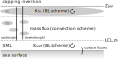
\includegraphics[width=0.7\textwidth]{chapter4/fig/scheme.pdf}
\caption[A scheme showing the operation of the boundary layer and convection schemes]{A scheme showing the operation of the boundary layer (BL)
and convection schemes in a cumulus (Cu) below stratocumulus (Sc) profile
commonly observed in the summertime Southern Ocean. Surface mixed layer (SML),
lifting condensation level (LCL).
}
\label{fig:4:scheme}
\end{figure}

Figure \ref{fig:4:scheme} show a schematic of operation of the UM11.4 boundary layer and convection
parametrisation most
commonly occurring during the TAN1802 voyage in situations with Sc cloud,
and Table \ref{tab:4:levels} summarises the BL diagnostic levels of the model.
This situation corresponds to the BL Type V in \cite{lock2000} (decoupled Sc over Cu).
In the UM11.4 this is parametrised by the BL scheme first-order turbulence scheme
in the surface and Sc layers and the convection scheme mass flux parametrisation
between these two layers. The level separating the surface turbulence and
mass flux is the LCL, above which moist convection is expected to occur.
As noted by \cite{lock2000}, this vertical separation of the parametrisation
schemes is undesirable, but also unavoidable due to the BL scheme partially
accounting for the vertical transport by convection. As we will show later,
this vertical separation of the two parametrisation schemes may be responsible for the
lack of Sc in the model compared to observations (Sect. \ref{sec:4:bl-mass-flux-and-rh}). For the purpose of BL
cloud simulation, we are chiefly concerned with the vertical moisture and air
mass transport from the sea surface to the Sc layer. This process is simulated
by:

\begin{enumerate}
\item A flux of moisture from the sea surface to the surface layer, determined
by the sea surface roughness in the surface scheme (JULES).
\item Mixing of moisture and heat in the SML by turbulence up to the LCL.
\item Flux of mass and moisture by convection from the LCL to the capping inversion.
\item Forced detrainment of air mass from the convective updraft into the environment
below the capping inversion (corresponding to the $z_{par}$ level),
identified in the model as the capping level for a moist lifted parcel.
\end{enumerate}

If these processes are sufficient, enough moisture (saturated air) is detrained
below the capping inversion to increase RH above the critical RH and condense the
excess water vapour into Sc cloud. Deficiencies in any of above processes or their interconnections can result in a deficiency in RH and a lack of Sc compared to observations. Our aim is therefore to identify which of these processes or interconnections are underestimated.

\begin{table}
\caption[Diagnostic model levels and layers]{
Diagnostic model levels and layers relevant to shallow boundary layer convection, turbulence
and cloud, listed from the lowest to the highest.
}
\label{tab:4:levels}
\centering
\scalebox{0.71}{
\begin{tabular}{llllllll}
\hline
Level & Description\\
\hline
SL (surface layer) & Layer between the surface and the lower of 0.1$z_h$ and level where $\theta_{vl}$ starts to increase with height.\\
SML (surface mixed layer) & Turbulently well-mixed layer between the surface and the LCL.\\
LCL (lifting condensation level) & Traditional definition (e.g. \cite{wallace2006}).\\
$z_h$ & Level equal to the LCL if cumulus-capped, or $z_{par}$ if not.\\
$z_{par}$ & Top of a diagnostic moist parcel ascent.\\
\hline
\end{tabular}
}
\end{table}

\subsection{Experimental run}
\label{sec:4:experimental-run}

We prepared an experimental run of the UM11.4 ("UM11.4exp") in order
to evaluate the effect of tuning of the processes outlined in Sect. 
\ref{sec:4:schemes} on the simulation of Sc in the Ross Sea to compare
with the TAN1802 voyage observations. 
In order to increase the moisture transport from the surface to the sub-capping-inversion layer, we applied the configuration and code modifications described below:

\begin{itemize}
\item We used the fixed sea surface roughness length option
(Sect. \ref{sec:4:jules}) with a fixed scalar surface roughness length of $10^{-4}$
m. This value is approximately equal to the maximum in the empirical
fit of COARE data \citep{fairall2003}. The motivation for this change is to increase
the surface flux of moisture to the greatest physically meaningful value.
\item We increased a coefficient relating sub-cloud convective velocity scale
to cumulus mass flux for shallow convection ($c_\text{mass}$) by 50\%. 
$c_\text{mass}$ determines the initial mass flux in the surface buoyancy
flux closure (Sect. \ref{sec:4:convection-scheme}). This has the effect
of increasing the initial mass flux by 50\%. The motivation for this change
is to increase the speed of convective updrafts, by which the forced
detrainment of saturated air below the capping inversion is increased.
\end{itemize}

\section{Results}
\label{sec:4:results}

In this section we compare the experimental run UM11.4exp described in Sec. \ref{sec:4:experimental-run} with the control run UM11.4cnt, in-situ observations on TAN1802 and satellite observations from the CERES instruments' synoptic (SYN) product \citep{loeb2018} in the time period between 16 February 2018 and 15 March 2018.

\subsection{Cloud observations}

\begin{figure}[p]
\centering
\includegraphics[width=\textwidth]{chapter4/fig/backscatter_rs.pdf}
\caption[Selected daily backscatter profiles collected on the TAN1802 voyage
and radiosonde profiles]{Selected daily backscatter profiles collected on the TAN1802 voyage
and radiosonde profiles. Shown are the lifting condensation level (LCL),
sea surface temperature (SST) lifting level (SLL) and SST lifting level for a saturated parcel (SLL$_s$).
Radiosonde launch times are indicated by a vertical line on the backscatter
plots and the height of the LCL, SLL and SLL$_s$ is indicated by a coloured dot.
}
\label{fig:4:backscatter-rs}
\end{figure}

As shown previously by \cite{kuma2020a}, the BL cloud base in the SO commonly
corresponds to either the LCL or the SST lifting level (SLL). Here, we show
that in the TAN1802 voyage observations, three clouds layers were often observed
and corresponded to three different thermodynamic levels. Figure
\ref{fig:4:backscatter-rs} shows several days of co-located ceilometer and
radiosonde observations. Based on the radiosonde profiles, we calculated the
following thermodynamic levels: the LCL, SLL and saturated SLL (SLL$_s$), which
uses the same assumption as SSL, but allows the parcel to ascend by moist
adiabatic processes above the LCL. On a majority of days with Sc cloud, we observed
that the LCL corresponded with the cloud base of relatively thin Cu fractus
below 1 km ASL (visible on all days in Fig. \ref{fig:4:backscatter-rs}). The much thicker
layer of Sc corresponded with SLL between 1 and 2 km ASL, i.e. due to parcels lifted by dry convection.
In several cases, SSL$_s$ corresponded with a third layer of cloud above Sc
(Fig. \ref{fig:4:backscatter-rs}a, d, e), i.e. due to parcels lifted by moist
convection. The third layer was, however, intermittent and much less significant
than the Sc cloud based identified near SLL. Examination of radiosonde profiles, shows that SLL and SLL$_s$ were both characterised by an inversion (most clearly visible in Fig.
\ref{fig:4:backscatter-rs}e'). Physically, this inversion would act to prevent
further ascent of a parcel and cause a forced detrainment of convective updrafts,
thus leading to accumulation of moisture below the inversion and the gradual
formation of Sc cloud. As discussed later, we think that this process is
underestimated in the UM11.4, which explains the absence of Sc layers in the model compared to observations.

\subsection{Cloud representation}
\label{sec:4:cloud-representation}

\begin{figure}[p]
\centering
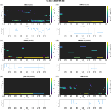
\includegraphics[width=\textwidth]{chapter4/fig/examples.pdf}
\caption[Selected daily observed and simulated backscatter profile plots]{Selected daily observed and simulated backscatter profile plots.
The observations (OBS) were collected on the TAN1802 voyage and the
simulations are based on the UM11.4 control (UM11.4cnt) and experimental (UM11.4exp) runs
at the same time and geographical location as corresponding the observations.
The plots also show the radiosonde lifting condensation level (LCL), sea surface temperature (SST) lifting level (SLL), saturated SST lifting level (SSL$_s$), the model LCL, diagnostic parcel height (z$_{par}$) and
updraft detrainment rate (DTRU). The vertical extent is limited to 5 km ASL.
}
\label{fig:4:examples}
\end{figure}

\begin{figure}[t]
\centering
\includegraphics[width=\textwidth]{chapter4/fig/examples_cont.pdf}
\caption{Figure \ref{fig:4:examples} continued.
}
\label{fig:4:examples-cont}
\end{figure}

A characteristic feature of the SO cloud observed on the TAN1802 voyage
by a ceilometer
were layers of relatively optically thick, but geometrically thin Sc
at between 1 and 3 km ASL (Fig. \ref{fig:4:backscatter-rs}, \ref{fig:4:examples}
and
\ref{fig:4:examples-cont}; in particular Fig. \ref{fig:4:examples}a1 17:00--0:00, b1 0:00--12:00, c1
4:00--9:00, e1 12:00--20:00, Fig. \ref{fig:4:examples-cont}a1 0:00--4:00).
These were commonly accompanied by Cu fractus
below the Sc layer. 
Apart from these two types of cloud, a significant amount
of fog was observed on the voyage (Sect. \ref{sec:4:cloud-occurrence-statistics}).
In Fig. \ref{fig:4:examples} and \ref{fig:4:examples-cont} we compare the
observed and simulated backscatter in the UM11.4cnt and UM11.4exp on
multiple days of the voyage, as well as the thermodynamic levels.
The selected days contain substantial amount of Sc cloud layers,
and we omitted days which were dominated by clear sky, fog and precipitation.
We note that
temporal and cloud height correspondence between the observations and simulations
is generally very good, partly due to the high temporal output resolution of
the model of 20 min \citep{kuma2020b}. Both are characterised by boundary
layer cloud below 2 km ASL, and this altitude corresponds very well with
the $z_{par}$ level diagnosed by the model, i.e. the highest level reached
by convection. Likewise, the LCL corresponds relatively well between the
radiosonde observations and the model (red dot in OBS vs. red line in the UM
in Fig. \ref{fig:4:examples} and \ref{fig:4:examples-cont}; see also \cite{kuma2020a}).
However, clouds simulated by the
UM11.4cnt are clearly different from observations in a number of ways.
While the periods of fog are relatively well simulated, the Cu fractus
cloud layers forming at and above the LCL are clearly overestimated in the
UM11.4cnt. Most seriously, the very well-defined Sc cloud layers are
completely absent in the UM11.4cnt, and are only represented by
intermittent vertical streaks of cloud instead of a coherent horizontal 
"stratiform" development. We can expect this factor to have a strong
impact on the SW radiation balance due to overestimated Cu reflectivity
and underestimated Sc reflectivity. Our aim with the experimental run is
therefore to improve
the simulation of Sc cloud as a major deficiency of the control run.

By increasing surface moisture flux in the UM11.4exp we increase
the amount of moisture in the surface layer, and by increasing mass
flux we in turn increase the amount of air mass and moisture transported
from the SML to $z_{par}$. The impact on the simulated
cloud backscatter is an increase in the amount of cloud just below $z_{par}$ (Fig.
\ref{fig:4:examples} and \ref{fig:4:examples-cont}),
which is more consistent with observations. Some of the more
prominent examples of an improved Sc are \ref{fig:4:examples}b3 3:00--9:00, c3 17:00--0:00,
e3 12:00--21:00 and Fig. \ref{fig:4:examples-cont}b3. A secondary effect
of the increased mass flux is a decrease of the simulated Cu fractus as
compensating convective downdrafts detrain warmer and drier air at the bottom
of the plumes near the LCL (for example Fig. \ref{fig:4:examples}b3 3:00--9:00, e3 12:00-20:00
and Fig. \ref{fig:4:examples-cont}a3, b3). This is potentially a positive
development considering the overestimated Cu fractus in the UM11.4cnt compared
to TAN1802 observations.

Figures \ref{fig:4:examples} and \ref{fig:4:examples-cont} also show contour lines
of the convective detrainment rate (DTRU) as diagnosed by the model's
convection scheme. These largely signify the forced detrainment from convective
updrafts of the mass flux scheme, whereby saturated air is removed from the
updraft and detrained into the environment, thus increasing RH.
Importantly, in the UM11.4cnt DTRU is locally concentrated in the vertical layer
where we expect Sc cloud. However, this is apparently not enough to raise RH beyond the critical RH to initiate sufficient Sc cloud formation (also discussed later in Sect.
\ref{sec:4:bl-mass-flux-and-rh}).
This indicates that the model is qualitatively correct in its representation
of the BL, but that the magnitude of the change is too small. In the UM11.4exp DTRU was expanded and intensified. 
This was likely the key contributor to the increased
Sc cloud, although a deficiency of this type of cloud persists in the
UM11.4exp.

% the difference between DTRU in the two runs is hard to see in the figures and is only visible (in my opinion) as an increase in the area and partially as a focusing in the region of DTRU contours. Can this be quantified better. Would changing the threshold for the contours help?  AJM

\subsection{Boundary layer mass flux and relative humidity}
\label{sec:4:bl-mass-flux-and-rh}

\begin{figure}[p]
\centering
\includegraphics[width=0.8\textwidth]{chapter4/fig/examples_hur_mcu.pdf}
\caption[Mass flux and relative humidity profiles]{Mass flux (odd rows) and relative humidity (even rows) profiles in the UM11.4 control (UM11.4cnt)
and experimental (UM11.4exp) runs, corresponding to the plots in Fig. \ref{fig:4:examples}.
}
\label{fig:4:examples-hur-mcu}
\end{figure}

\begin{figure}[t]
\centering
\includegraphics[width=0.8\textwidth]{chapter4/fig/examples_hur_mcu_cont.pdf}
\caption{Figure \ref{fig:4:examples-hur-mcu} continued.
}
\label{fig:4:examples-hur-mcu-cont}
\end{figure}

Model BL cloud in the UM11.4 is driven by the underlying process
of vertical moisture and air mass transport due to turbulence and convection
(which can in turn be driven by large-scale dynamics). The large-scale cloud
(PC2) scheme ensures that if enough RH is present in a particular model
layer, liquid or ice cloud condensation happens. We examined the BL mass
flux and RH in the UM11.4cnt and UM11.4exp on a number of days during the TAN1802
voyage (Fig. \ref{fig:4:examples-hur-mcu} and \ref{fig:4:examples-hur-mcu-cont}),
corresponding to days analysed in Sect. \ref{sec:4:cloud-representation}.
As explained in Sect. \ref{sec:4:schemes}, the mass flux parametrisation
extends vertically between the LCL and $z_{par}$. In this convective layer mass
flux is positive and transports air from the LCL to $z_{par}$ in updrafts
and from $z_{par}$ to the LCL in downdrafts. 
This corresponds with positive
DTRU just below $z_{par}$. In some instances, intermittent mass flux was
simulated by the UM11.4cnt (e.g. Fig. \ref{fig:4:examples-hur-mcu-cont}c1). This
is most likely related to the stabilisation of the layer by compensating
downdrafts, effectively shutting down convection until sufficient warm
and moist air is replenished from the surface layer. We hypothesise that this
may be an indication that the mass flux parametrisation operates more quickly 
than the surface turbulence with respect to moisture transport and therefore these two processes are not currently well-tuned to operate together. This appears to be the case in the unmodified
model, but is intensified further in the experimental run.

RH in the UM11.4cnt was characterised by two local peaks at the LCL and $z_{par}$
during periods when Sc cloud were observed. This is partially consistent
with the expectation of Sc occurring preferentially at $z_{par}$. This was, however, apparently not enough for sufficient cloud formation in this layer since RH is typically below 85\%.
In the UM11.4exp run, the positive mass flux extent was increased and intensified,
which resulted in a greater extent and intensity of DTRU. The problem of
mass flux intermittency was still present in the experimental run. The increased
mass flux had an obvious impact on RH, which separated the LCL and $z_{par}$
levels more clearly as two local peaks of RH, with a relatively dry
convective layer between these two levels. RH at $z_{par}$ was also increased,
and this lead to a greater formation of Sc cloud (Sect.
\ref{sec:4:cloud-representation}).  %Can we quantify this relative to observations or plot differences to highlight this point? AJM
However, the modifications in the UM11.4exp
did not appear to be sufficient to fully address the problem of underestimated
Sc cloud. RH at $z_{par}$ was still too low to enhance cloud formation in many cases, and our experiments with
increasing mass flux further (not shown) indicate that the mass flux
parametrisation cannot by itself solve the problem further. By a more extreme
tuning we also risk increasing mass flux to unphysical values.
Instead, the problem appears to be with the coupling of the surface layer
turbulence with the mass flux parametrisation, whereby not enough air mass
and moisture is transported across the LCL from the SML to the convection layer. In
other words, the BL scheme mixes moisture within the surface layer (up to the LCL)
by turbulence and the convection scheme transports air between the LCL and
$z_{par}$ by updrafts and downdrafts, but there is too little flux across the LCL,
effectively decoupling the two schemes. Compared to our
radiosonde observations, the peak of RH in the SML seems unphysical and
produced artificially by the separation of the BL and convection schemes
into two distinct vertical sections.

% I would like to see a figure that quantifies the RH vertical distribution AJM

\subsection{Cloud occurrence statistics}
\label{sec:4:cloud-occurrence-statistics}

\begin{figure}[t]
\centering
\includegraphics[width=0.5\textwidth]{chapter4/fig/cloud_occurrence.png}
\caption[Cloud occurrence histogram as a function of height]{
Cloud occurrence histogram as a function of height calculated from
28 days of the TAN1802 voyage calculated from ceilometer observations (OBS),
simulated lidar data in the control run of the UM11.4 (CNT) and
the experimental run of the UM11.4 (EXP).
Shown is also the total cloud fraction.
}
\label{fig:4:cloud-occurrence}
\end{figure}

While the case-based comparison of observed and simulated backscatter
shows an improvement of Sc cloud simulation, it is important that the impact
on the long-term cloud occurrence statistics is positive. We analysed
cloud occurrence by height as determined by a cloud masking algorithm
applied to the backscatter profiles \citep{kuma2020b}.
Figure \ref{fig:4:cloud-occurrence} compares cloud occurrence in observations,
the UM11.4cnt and UM11.4exp runs. The observed cloud peaked near the surface due to
the frequent fog occurrence previously discussed in \cite{kuma2020a},
with two smaller peaks at about 500 m a 1 km ASL due to Sc cloud.
Mid-level and high cloud above 2 km ASL was insignificant, probably due
to observational constraints (lidar signal fully attenuated by fog and low
cloud). The total cloud (+fog) fraction was observed to be 95\%.
The UM11.4cnt represented the statistical cloud occurrence remarkably well,
especially of fog, but possibly overestimated cloud below 2 km ASL. Considering
the results of the case study approach (Sect. \ref{sec:4:cloud-representation}), we think this is related to the
overestimation of Cu cloud in the model. The peaks related to Sc cloud were not present in the UM11.4cnt, as one would expect from the lack of Sc cloud
visible on the daily backscatter plots. The UM11.4exp showed a very similar
cloud occurrence as the UM11.cnt, with the exception of a much stronger peak which we believe is  associated with the Sc cloud at about 1.5 km ASL. Therefore, the modifications
in the UM11.4ext had the desirable effect of increasing Sc cloud statistically,
but the overall pattern of vertical cloud occurrence is not substantially better
than in the UM11.4cnt simulation. The total cloud fraction in the UM11.4exp was marginally
improved at 93\% (relative to observed 95\% and control of 91\%).

% I think highlighting that this was an aim would be useful. I also think identifying that previous work by Schuddeboom et al. (2019) and many others has highlighted that the cloud type is often wrong even if the cloud fraction is right. So this increase in cloud associated with enhancements in the SC type is actually potentially also partially removing a compensating error might be useful.

\subsection{Shortwave radiation bias}
\label{sec:4:sw-bias}

\begin{figure}[t]
\centering
\includegraphics[width=\textwidth]{chapter4/fig/sw.png}
\caption[Top of atmosphere outgoing shortwave radiation]{Top of atmosphere outgoing shortwave radiation in CERES SYN (OBS) and
bias in the UM11.4 control (UM11.4cnt) and experimental (UM11.4exp) runs relative
to CERES SYN during the period of TAN1802 observations 16 February--15 March 2018.
\textbf{(a, d)} show absolute values and \textbf{(b, c, e, f)} show values relative
to CERES SYN. The top row \textbf{(a--c)} shows the whole globe, the bottom
row \textbf{(d--f)} shows the Southern Ocean specifically.
}
\label{fig:4:sw}
\end{figure}

While the modifications in the UM11.4exp were aimed at achieving a better
match with lidar observations of BL cloud, these are also expected to
result in an improved TOA radiation balance due to the strong effect of
clouds on the planetary albedo. Figure \ref{fig:4:sw} shows the absolute
and relative reflected SW radiation in CERES, the UM11.4cnt and UM11.4exp
during the time period of in-situ observations. Similar to previous
versions of the UM \citep{kuma2020a,schuddeboom2019}, the bias in the UM11.4cnt
in the SO is characterised by a bipolar zonally-symmetric pattern of negative
biases in the high-latitude SO
and positive bias in the low-latitude SO (Fig. \ref{fig:4:sw}e).
As shown in our previous multi-voyage ceilometer
evaluation \citep{kuma2020a}, this is likely caused by the "too few, too bright"
cloud problem. The experimental run displays an improved SO SW radiation
bias, especially by unexpectedly reducing the positive bias in the low-latitude SO
(Fig. \ref{fig:4:sw}f). Globally, the bias in the UM11.4cnt was positive in most
regions (Fig. \ref{fig:4:sw}b). This has been reduced in the UM11.4exp, without
a significant deleterious impact on the existing regions of negative bias. We stress,
however, the limited time period of the comparison (16 February--15 March 2018).

The zonal average of the TOA SW bias over the time period of the in-situ
observations shows mostly positive bias in the
UM11.4cnt, peaking at about 24 \unit{Wm^{-2}} near the equator (Fig. \ref{fig:4:sw-zonal}). In the
UM11.4exp the bias is reduced by up to 5 \unit{Wm^{-2}}, with most
latitudes experiencing a reduction of bias. Surprisingly, the southern
part of the SO was largely unchanged, despite the improvement in the
representation of the Sc cloud relative to the in-situ observations.

\subsection{Boundary layer types}
\label{sec:4:bl-types}

% I think an introductory sentence at the start of this paragraph highlighting why you are doing this is necessary.

The BL scheme classifies a grid cell as one of six grid cell BL types
(Sect. \ref{sec:4:bl-scheme}). In the UM11.4cnt in the time period of the in-situ observations,
the most frequent BL types in the SO were Type I (stable BL) and V (decoupled Sc
over Cu), peaking at about 80 and 90\% in some regions of the SO, respectively
(Fig. \ref{fig:4:bdyt}a, e).
Type I was prevalent mostly in the low-latitude SO, while Type V was
prevalent primarily in the high-latitude SO. This difference might partially explain
the different SW radiation bias of these two zones (Sect. \ref{sec:4:sw-bias}). % Can you explain why? AJM
In the UM11.4exp, the distribution of BL types has significantly changed
globally relative to the control run (Fig. \ref{fig:4:bdyt}g--l). The most significant change in the SO
was the increase in the occurrence of Type V in both the low- and high-latitude SO (Fig.
\ref{fig:4:bdyt}k), while Type I had a minor increase in the SO (Fig.
\ref{fig:4:bdyt}g). This suggests that the increase of Type V in the low-latitude
SO might be associated with the improved SW radiation bias in this zone.

\section{Discussion and conclusions}
\label{sec:4:conclusions}

\begin{figure}[p]
\centering
\includegraphics[width=0.8\textwidth]{chapter4/fig/sw_zonal.pdf}
\caption[Zonal average of top of atmosphere outgoing shortwave radiation]{
Zonal average of top of atmosphere outgoing shortwave radiation in
the UM11.4 control (UM11.4cnt) and experimental (UM11.4exp) runs relative
to CERES SYN during the period of TAN1802 observations 16 February--15 March 2018. 
}
\label{fig:4:sw-zonal}
\end{figure}

\begin{figure}[p]
\centering
\includegraphics[width=\textwidth]{chapter4/fig/bdyt.png}
\caption[Boundary layer type histograms]{Boundary layer type histograms of Type I--VI \citep{lock2000} in the UM11.4cnt
\textbf{(a--f)} and UM11.4exp relative to the UM11.4cnt \textbf{(g--l)} expressed as percentage point (pp)
difference.
}
\label{fig:4:bdyt}
\end{figure}

We analysed 28 days of voyage data in the Ross Sea and identified a common
three-layer cloud profiles composed of Cu fractus, Sc and occasional
Ac, associated with the thermodynamic levels LCL, SLL and SLL$_s$, respectively.
This suggests a strong role of thermodynamics in the SO BL cloud formation.
We analysed a control run of the UM11.4 in comparison with ceilometer
observations using a lidar simulator framework. We found Sc cloud grossly
underrepresented in the model, indicating that the current BL and convection
schemes are not able to simulate this type of cloud. Considering these results,
we prepared an experimental run which increased the amount of moisture flux
from the sea surface and increased the convective mass flux, in order to
generate more Sc by increasing RH at the top of the BL. We showed that this
experimental run was more successful in simulating Sc, but other
modifications are likely needed to achieve a satisfactory correspondence with
the observations. The experimental run showed a greater ability to couple the
surface with the top of the BL, but the connection between the BL and convection
scheme appears to be too weak to allow sufficient transport of air mass and
moisture across the LCL. Therefore, the artificial vertical separation of operation of the
BL and convection schemes to surface--LCL and LCL--z$_{par}$ regions appears
to hinder the transport of moisture across the LCL, and to the top of the BL.

We showed that the experimental run not only improves Sc cloud in the Ross Sea,
but also improves the SW radiation balance in the SO, especially in the
low-latitude SO north of 60$^\circ$S. In other parts of the globe the effect was
also positive, with a decrease of zonal SW radiation bias of up to 5
\unit{Wm^{-2}} by reducing the common positive bias of the model. The
effect on the BL types are primarily switching from the stable BL Type I
to the convective Type V (Sc over Cu) across the whole of the SO. % so why don't we see a bigger difference consistently?
Currently we do not suggest that the tuning in the experimental model is
integrated into the main model due to the modifications being relatively
extreme. Our results, however, suggest that if the
coupling between the BL and convection schemes across the LCL is improved,
either more minor or no tuning would be required to obtain sufficient moisture
transport from the surface to the top of the BL for Sc cloud formation.
The SW radiation bias results indicate that the effect on the rest of the
globe might be positive rather than negative, which would be otherwise
expected if only one region (the Ross Sea) is taken into consideration in any
tuning of the model. We also showed that a ground-based lidar simulator
applied on high temporal resolution model output can be a useful tool for an
analysis and improvement of BL cloud using a case study approach.

% I think the discussion part of this section needs to be strengthened, it appears to me that you have highlighted a good set of conclusions. But, I am not sure your discussion points come out - I would try to find references which support your more speculative statements. I think the disconnect between layers is quite clear, but are there other papers which have highlighted this mismatch?  AJM

%\codeavailability{TEXT}
%\dataavailability{TEXT}
%\codedataavailability{TEXT}
%\sampleavailability{TEXT}
%\videosupplement{TEXT}

\small
\sffamily

\subsection*{Author contributions}

Peter Kuma participated on the TAN1802 field measurements, performed the model runs, analysis and wrote the manuscript;
Adrian McDonald organised the deployment of instruments on the TAN1802 voyage and participated on continuous discussion of the analysis
and manuscript;
Olaf Morgenstern participated on continuous discussion of the analysis and
manuscript;
Sean Hartery participated on the TAN1802 field measurements;
Jonny Williams, Vidya Varma and Guang Zeng contributed substantially to the
nudged UM setup;
Mike Harvey organised the deployment of instruments on the TAN1802 voyage;
Simon Parsons and Graeme Plank participated on the deployment of instruments on the TAN1802
voyage. All authors reviewed the manuscript.

\subsection*{Acknowledgements}

We would like to acknowledge the contributions of those who participated on
the TAN1802 voyage and deployment, especially the crew of the voyage;
Alex Schuddeboom for reviewing the manuscript; the UK Met
Office for providing the HadGEM3-GA7.1/UM11.4 model;
the CERES project for providing publicly available data via the NASA Langley
Research Center CERES ordering tool (\url{https://ceres.larc.nasa.gov});
the
NeSI high-performance computing facilities
provided by the NZ eScience Infrastructure and funded jointly by NeSI's
collaborator institutions and the Ministry of Business, Innovation \&
Employment's Research Infrastructure programme (\url{https://www.nesi.org.nz});
the financial support of the Deep South National Science Challenge via the Clouds and
Aerosols project; the open source software we used to produce this analysis: Python, R,
numpy, scipy, matplotlib,
netCDF4, Linux and Devuan GNU/Linux.

\normalfont
\normalsize

\chapter{Conclusions and further work}

We conducted ship-based observations on the 2-week long voyage TAN1702 of
RV \textit{Tangaroa} to the Campbell Plateau
in March 2017 and the 6-week long voyage TAN1802 of RV \textit{Tangaroa} to the Ross Sea
in February--March 2018. These included ceilometer, lidar, radar, radiosonde,
sky camera, automatic and human weather observations and aerosol measurements.
We deployed ceilometers, radar and a sky cameras on additional voyages:
the December 2016 voyages of HMNZS \textit{Wellington} and an 
April--May voyage NBP1704 of RV \textit{Nathaniel B. Palmer} to the Ross Sea.
In addition we collated and processed observations from previous voyages
of \textit{Aurora Australis}, TAN1502, TAN1503 and land-based ceilometer
observations on Macquarie Island.
We set up and performed nudged simulations
of the Global Atmosphere version 7.1 (GA7.1) on a supercomputer of the New Zealand eScience Infrastructure (NeSI) and the National Institute of Water \& Atmospheric Research (NIWA).
We compared the model output with our collection of ship-based observations,
focusing on geometrical properties of clouds observed by ceilometers and their
links to thermodynamical profiles of the atmosphere observed with radiosondes.
We contrasted these with the MERRA-2 reanalysis. Both the nudged GA7.1 and MERRA-2
showed significant cloud occurrence biases of 4--18\% less cloud than in
ceilometer observations. Despite of this, both showed a bipolar shortwave (SW)
radiation
bias by latitude, with outgoing SW radiation underestimated in high-latitude
SO and overestimated in low-latitude SO. This suggests that compensating biases
of cloud occurrence vs. cloud optical thickness are present in the models.
This bipolar SW radiation bias was strongly correlated with near-surface air temperature,
with relatively low air temperature regions exhibiting a negative SW radiation bias and
relatively high temperature regions exhibiting a positive SW radiation bias. By analysing
lifting levels, lifting condensation level (LCL) and the level of neutral buoyancy
of an air parcel with potential temperature equal to sea surface temperature (SST),
we showed that cloud base in the region is strongly linked to these levels,
and these levels were a better predictor for cloud base than the previously
utilised lower tropospheric stability (LTS). This finding suggests that local
thermodynamics is a strong driver of the summertime SO stratocumulus (Sc) clouds,
a finding also supported by \cite{hartery2020b}. Interestingly, we found
very large differences in cloud phase simulated by the nudged GA7.1 and MERRA-2.
MERRA-2 simulated much greater amount of liquid cloud (the majority of
the water path), while the GA7.1 simulated slightly more ice than liquid.
Even though we did not use an observational reference for cloud phase,
we can say that the cloud phase was most likely behind the difference in
cloud biases between the GA7.1 and MERRA-2 (in addition to the identified cloud occurrence biases), which were much more positive
in MERRA-2 (liquid cloud reflects more SW radiation for the same amount of water
path). We conclude that cloud geometry biases play at least an equally
significant role in radiation biases as cloud phase and these two can be
compensating biases, a fact which was not given enough recognition in previous
studies. The source of the bipolar biases and its strong relationship with
near-surface temperature, however, is still relatively unclear.

In order to compare ceilometer and lidar observations with models,
we developed the Automatic Lidar and Ceilometer Framework (ALCF),
a tool which extends the Cloud Feedback Model Intercomparison Project (CFMIP) Observation Simulator Package (COSP) lidar simulator with support for a range
of ground-based instruments and a processing pipeline which allows
for an unbiased comparison of simulated and observed backscatter and a cloud mask.
This tool was the subject of Chapter 3. While the COSP lidar simulator
provided a basis for the physical simulation of laser radiation transfer
through the atmosphere, more work needed to be done to support the ground-based
instruments with their variety of field of view (FOV), wavelengths and
calibration issues. By developing and documenting this tool, we enabled future
studies utilising off-the-shelf ground-based lidars for model evaluation.
The potential of ground-based lidars has so far been underutilised compared
to similar active satellite observations (CALIPSO) due to the
lack of software processing tools and the difficulty of accurate calibration
of these instruments. The problems addressed by our work included Mie
scattering at different laser wavelengths depending on droplet size distribution
parameters, absolute calibration by utilising Sc clouds and molecular
backscattering, backscatter noise removal, cloud mask/cloud base determination 
and evaluation of noise characteristics of various common lidars. We demonstrated
usefulness of this new tool on several case studies. Several common atmospheric
models and reanalyses are supported by this framework, which allowed us to compare
a range of publicly-available model output with ceilometer and lidar observations
at several stations in Aotearoa/New Zealand. We showed how this tool can be used
for comparing vertical cloud occurrence, backscatter "curtain" plots
and cloud fraction vs. optical thickness. More processing algorithms can
be incorporated in this modular tool in the future to allow for calculation of
derived products.

Lastly, we focused on evaluation of SO boundary layer cloud in the GA7.1
and how the BL turbulence and convection parametrisations affect
BL cloud. Previously, we found that Sc cloud below 2 km above sea level (ASL)
and fog were predominant in the SO, but underestimated in the model. We used
the ceilometer observations collected on TAN1802 to evaluate the model cloud
in a case study based approach, where we compared "curtain" backscatter plots
between the model and observations using the ALCF. This allowed us to identify
in detail that the model is missing the extensive layers of Sc cloud found
in observations, while overestimating cumulus (Cu) clouds occurring below the
Sc layers. In observations, these layers were found to correspond to LCL (Cu clouds),
and the level of dry and moist neutral buoyancy of a parcel with potential temperature
equal to SST lifted from the sea surface (Sc clouds). Therefore, BL
thermodynamics was identified as being key to resolving these biases. By running
a model experiment with an increased surface flux and mass flux, we tested
a hypothesis that not enough moisture transport is simulated to accumulate
moisture at the top of the BL for cloud condensation. When compared with
observations, this experiment lead to an improved occurrence of Sc clouds,
but due to a limiting factor we were unable to attain a full correspondence
with observations. We identified the coupling between the turbulence and convection
parametrisations across LCL as the most likely bottleneck. Therefore, it seems
that the separation of parametrisation into turbulence and convection driven
vertical regions appears to limit the formation of Sc clouds in the BL in the
summertime SO. Our experimental run showed promising results in terms of
SW radiation biases globally (evaluated on a short monthly time period in February--March 2018),
where the zonal means were reduced by up to 5 Wm$^{-2}$. We conclude that
further modifications to the BL schemes are needed to improve
Sc cloud simulation in the SO. The tuning in the experimental run also needs to
be evaluated globally over a long time period to determine if it can be used
operationally. This approach when individual clouds can be compared between
a nudged model and observations means that compensating biases are avoided.
Secondary to this approach should be evaluation of cloud optical thickness,
cloud phase and the cloud--aerosol effects, which all contribute to the
radiation biases. In this sense, our work is complementary to that of
\cite{revell2019}, \cite{hartery2020a} and \cite{hartery2020b}.

We can summarise our contributions as follows. The relatively large SO
cloud biases and the resulting radiation biases are still common in GCMs
and reanalyses today \citep{gettelman2020}. Due to the relatively large
extent of the SO, its role in the uptake of excess heat and CO$_2$
and being a buffer zone for warming of the Antarctic ice sheets, and the Southern Hemisphere
meridional circulation, it has a crucial role in the Earth's climate system.
Clouds are the major factor in Earth's albedo variability. Therefore, any cloud
biases can result in large biases in a model's large scale atmospheric
and oceanic circulation and the cryosphere. Unless these biases are minimised
in GCM simulations of the past and present climate, the accuracy of future climate
simulations is limited, especially when it comes to predicting the change
of cloud cover, the Earth's albedo, circulation and the ice sheets.
Using ship-based observations, we narrowed down the cloud climatology
in the SO, its main drivers and factors involved in the cloud biases. We
identified BL parametrisations of turbulence and convection as a major deficiency
in the model, and suggested concrete improvements. This work can translate into
eventually improving these parametrisations. The improved understanding of the
drivers can be applied in the development of other GCMs and reanalyses.
Development of the ALCF as a tool for evaluation of models using ground-based
lidar observations can streamline the process of using these type of observations
globally, and provide a unique opportunity to evaluate BL clouds, some of
which are not visible with spaceborne instruments. This new tool substantially
lowers the bar for utilising these instruments, and therefore it can enable
future studies of BL clouds.

\section{Further work}

Even though we analysed a large part of the ground-based SO observations
available to us (Chapter 2), they are still underutilised. For example,
we have not analysed the dual-polarisation lidar data collected on TAN1802
by a MiniMPL. If properly calibrated, these could provide crucial information
about supercooled liquid cloud. The micro rain radar (MRR-2) deployments
have so far been underutilised. They allow for detection of precipitation,
rain rate and vertical velocity in precipitation.
With analysis of the raw data it is also possible to get measures of snowfall
rate and their related vertical motion which is more variable than rainfall.
Model evaluation of
precipitation is needed to complement cloud evaluation in order to make
sure the right amount of moisture is being removed from the BL by precipitation
and the precipitation has the correct phase (liquid or ice). Similar to clouds,
precipitation has an effect on shortwave (SW) and longwave (LW) radiation. It is therefore important
for the radiation balance, considering its frequent occurrence in the SO.
A dual camera setup was installed on the TAN1802 voyage in order to allow
for stereoscopic determination of cloud base height. This imagery has not been
utilised so far, but a co-authored study has utilised sky camera images collected
on the \textit{Aurora Australis} voyages in comparison with
ceilometer observations \citep{klekociuk2018}.
Co-location with the ceilometer observations provides an
opportunity for algorithm development and cross-validation of results.
Likewise, cloud type and cloud fraction can be determined from sky camera
imagery using a suitable algorithm. A pair of sky cameras could be utilised as
a low-cost instrument for determining cloud base height, cloud fraction
and cloud type on ships of opportunity \citep{klekociuk2018}.

As we identified, ground-based observations have a large additional value
to satellite observations when it comes to BL cloud evaluation. More
ground-based observations in the SO could narrow the spatial and temporal gaps
in our understanding of the region. Therefore, making ship-based atmospheric
observations more accessible is an important task. Currently, deployment
of instruments such as lidar and radars on ships is logistically difficult
and expensive. Smaller and less expensive instruments could mean that they
can be deployed more widely and installed permanently on some ships. Smaller
lidars typically have lower power and inferior noise characteristics,
but a wide coverage could outweigh these deficiencies. Progress in lidar
development could also mean smaller instruments may become equally powerful.
The commercial nature of common instruments means that some instruments
suffer from a number of technical problems and vendors typically show
little interest in resolving these. Open hardware and open software design of
instruments could substantially accelerate progress and collaboration.
Off-the-shelf software defined radio (SDR) receivers and
transceivers\footnote{\url{https://limemicro.com}.} have recently
become widely available. They could provide a basis for development of improved
radars which can utilise many frequencies. Open software for processing
instrument data could mean that implementation of standard techniques and
algorithms for calibration, resampling, noise removal and calculation of derived
products become more available to the scientific community. Likewise,
public sharing of ground-based observational data and building of dataset
collections, similar to the common practice of releasing satellite datasets,
has a potential to accelerate atmospheric research in the SO.
Utilising unusual platforms such as the Argo floats \citep{roemmich2009}
as platforms for atmospheric measurements could provide a vast amount of data and a relatively dense
coverage in the SO.
Air--sea surface fluxes appear to be implicated in the GA7.1/UM11.4 cloud biases
(Chapter 4). Yet, the Coupled Ocean–Atmosphere Response Experiment (COARE)
formulas are potentially not well-tuned for high latitudes and atmospheric
reanalyses exhibit large air--sea flux biases in the SO
\citep{cerovevcki2011}. Evaluation of model air--sea flux biases relative to
reliable in situ flux measurements is needed to make sure they are not
a major cause of the BL cloud biases. Other related biases are in the
representation of marine aerosols, which act as a source of cloud condensation
nuclei (CCN) and ice nucleating particles (INPs) \citep{hartery2020a}.

A reliable comparison of models and observations using a lidar simulator
requires accurate absolute calibration of the observed backscatter
(Chapter 3). We have identified various deficiencies in the vendor-supplied
calibration such as the dead time, afterpulse and overlap calibration in
the MiniMPL. These often result in range-dependent bias of the volume
backscattering coefficient, which may be impossible to reliably correct
for without dedicated calibration measurements. Currently, the ALCF only
supports height-independent calibration utilising observations of liquid
Sc clouds and comparison with a theoretically expected
molecular backscatter (Chapter 4). An automated approach should be developed to calculate
dead time, afterpulse and overlap corrections as an alternative to the 
vendor corrections, which appear to be unreliable. This could lower the
difficulty of utilising ceilometer and lidar data by the wider scientific
community, which is a significant barrier for a wide utilisation of ceilometers
and lidars for model evaluation.
Currently, the ALCF does not support calculation of cross-polarised
backscatter. Adding support for simulation of cross-polarised backscatter
would mean that both channels of the Sigma Space MiniMPL can be utilised
in a comparison with a model and therefore evaluate cloud phase.
Likewise, aerosol and precipitation is currently not taken into account
by the lidar simulator. This not only causes a systematic bias in comparison
with observations, but also prevents the simulator being used for
model aerosol and precipitation evaluation.

A large amount of automatic lidar and ceilometer (ALC) data have been collected by regional and global
networks such as Cloudnet \citep{illingworth2007},
E-PROFILE \citep{illingworth2018}, EARLINET
\citep{pappalardo2014}, ICENET \citep{cazorla2017} and MPLNET
\citep{welton2006}. Most of these networks utilise ceilometers
and lidars already supported by the ALCF such as Vaisala CL31, CL51, Lufft CHM
15k and Sigma Space MiniMPL. These observations haven't been used
extensively for model evaluation. There is a potential to process and compare
these observations with models using the ALCF. Such comparison would complement
past comparisons with satellite observations, and could rival satellite
observations in terms of global spatial and temporal coverage. 

Here, we utilised the Clouds and the Earth's Radiant Energy System (CERES) satellite observations of top of atmosphere (TOA) radiation. Even
though the errors of these observations may be relatively low compared to 
current model cloud biases, systematic errors in the dataset exist due
to unequal diurnal sampling and the need for temporal and angle
interpolation of the raw measurements to calculate daily averages. 
The relatively new instrument National Institute of Standards and Technology
Advanced Radiometer (NISTAR) on the L1-stationed Deep Space Climate Observatory (DSCOVR)
provides a unique viewpoint for Earth radiation observations, from which 
the sunlit part of the Earth, including polar latitudes, is visible continuously.
It would be valuable to compare model radiation fluxes with these new
observations to rule out the effect of systematic biases of CERES on the
model TOA radiation evaluation.

An unresolved question about the origin of the bipolar SW radiation
bias in the high- and low-latitude SO in GA7.1 remains. We know that
the model underestimates low cloud, and at the same time, we identified
some evidence that the optical thickness of individual clouds is overestimated.
This may be the underlying reason for the overestimated reflected TOA SW
radiation in the low-latitude SO.

We identified that BL parametrisation of mass flux can be tuned
to enable Sc cloud simulation in the SO (Chapter 4). However,
a good observational reference for mass flux and the similarity relationships
is lacking in the SO. The BL turbulence and convection
parametrisation is based on large eddy simulations (LES) initialised
from field experiments in the tropical and midlatitude ocean. These may be
inappropriate for the SO. Therefore, new LES initialised from SO field
experiments are needed to make sure these parametrisations are correct in this
region.

We have shown that nudged simulations of GA7.1 provide a very good basis
for identifying model biases compared to ground-based observations. As opposed
to a free-running model, it can be reasonably assumed that any biases are
not the result of a different weather situation simulated by the model
than in reality, and that they are largely due to errors in the subgrid-scale
parametrisation processes not assimilated in the ERA-Interim reanalysis driving
the model or not an input to the model nudging algorithm. As shown in Chapter 4,
a side-by-side comparison of modelled and observed cloud is feasible, and this
can be utilised in future studies of model clouds.

In Chapter 2 we presented a dataset of ground-based observations in the SO.
This dataset provides a unique and comprehensive information on SO atmospheric
conditions and clouds. Work is underway to make this dataset documented and
publicly available. To this end, derived products should be developed in order
to make it easy for the scientific community to use this dataset. In general,
a more concentrated effort is needed to streamline public sharing of atmospheric
observations, especially considering the global and accelerating
effect of climate change, which has been called
"the defining challenge of our time" \citep{wmo2019} by the United Nations
Secretary-General A. Guterres. It is the author's opinion that the
seriousness and urgency of the situation is vastly underestimated even
by the atmospheric science community, which continues to hinder international
cooperation by not sharing data and model code, and by publishing scientific
results in paywalled journals, and therefore putting the well-being of future
generations in jeopardy. A question remains whether the parametrisations
can be formulated in a more physical manner without relying on the similarity
theory relations, which may not be universally applicable globally.

In Chapter 4 we identified that increasing convective mass flux and surface
heat flux can improve Sc cloud simulation. However, it remains
to be proven if mass flux or surface fluxes are underestimated relative to
a physical reference (either an observational reference or large eddy
simulations). More model experiments need to be performed which increase
flux between the turbulently-mixed surface mixed layer and the convective layer,
as well as longer term climate simulation to make sure the modifications
address the actual problem without introducing compensating biases,
and they do not have a negative impact on the
global radiation balance throughout the year. A new BL scheme "CoMorph"
is currently in development at the UK Met Office. Our findings could contribute
to the development of this new scheme, but more experiments need to be performed
with this new scheme and comparison of this new UK Met Office scheme with the ground-based
SO observations should be performed.

\clearpage

\footnotesize
\bibliography{introduction/bibliography,chapter2/bibliography,chapter3/bibliography,chapter4/bibliography,conclusions/bibliography}
\end{document}
